% ========================================================================
% TEMPLATE LATEX PARA TCC NO FORMTATO DE ARTIGO
% Baseado na classe abntex2 com personalizações para o IFPI
% Conforme e Manual de Normalização de Trabalhos Acadêmicos do IFPI - 2024 
% e as normas ABNT NBR:
%   14724:2011
%   6024:2012
%   6027:2012
%   10520:2023
%   6023:2018 
%   15287:2011 
% ========================================================================

% ========================================================================
% PREÂMBULO E CONFIGURAÇÕES
% ========================================================================

\input{config/config}   %configurações de formatação

\input{estrutura/dados}           %dados institucionais e do projeto

% ========================================================================
% INÍCIO DO DOCUMENTO
% ========================================================================

\begin{document}
% Seleciona o idioma do documento (conforme pacotes do babel)
\selectlanguage{brazil}
% Retira espaço extra obsoleto entre as frases
\frenchspacing

% ========================================================================
% ELEMENTOS PRÉ-TEXTUAIS
% ========================================================================
% ========================================================================
% ELEMENTOS PRÉ-TEXTUAIS
% Capa e folha de rosto conforme artigo TCC IFPI
% ========================================================================

% ========================================================================
% CAPA (Obrigatória em artigos do IFPI segundo o manual TCC)
% ========================================================================
\imprimircapa

% ========================================================================
% FOLHA DE ROSTO (Obrigatória)
% ========================================================================
\imprimirfolhaderosto*

% ========================================================================
% AGRADECIMENTOS (OPCIONAL - EM ARTIGOS DEVE IR NO FINAL)
% ========================================================================
% O manual do IFPI diz que agradecimentos em artigos vão como elemento pós-textual,
% portanto mude-os para o final do `main.tex` se for usar.

% ========================================================================
% CABEÇALHO DO ARTIGO (Título, autores, e-mails)
% ========================================================================
\imprimircabecalhoartigo

% ========================================================================
% RESUMO EM PORTUGUÊS E PALAVRAS-CHAVE
% ========================================================================
\setlength{\absparsep}{18pt} % Ajusta espaçamento entre parágrafos do resumo

\begin{resumo}
    O credenciamento manual de pacientes em instituições de saúde gera filas desgastantes, consome tempo excessivo e expõe o ambiente a vulnerabilidades de segurança e higiene. Para superar essas limitações operacionais, este artigo científico tem como objetivo desenvolver um artefato tecnológico de reconhecimento facial baseado em arquitetura de \textit{Edge Computing} para automatizar o processo de credenciamento de pacientes, reduzindo o tempo de espera e mitigando falhas operacionais. A metodologia utilizada baseia-se na \textit{Design Science Research }(DSR), com abordagem quantitativa e pesquisa experimental de campo. O sistema foi construído integrando um \textit{Single Board Computer} (SBC Labrador) a um módulo ESP32-CAM e sensores de distância (VL53L0X), operando de forma totalmente \textit{offline} e sem contato. O \textit{pipeline} de visão computacional utiliza as bibliotecas \textit{OpenCV} e \textit{Dlib} em conjunto com Redes Neurais Profundas para a extração de assinaturas faciais matemáticas (\textit{embeddings}). A fase de avaliação cruzou a \textit{baseline} empírica do processo manual nas clínicas — que registrou picos de espera de até 7 minutos e 51 segundos por paciente — com o desempenho em ambiente controlado do protótipo. Os resultados demonstram que o artefato conclui o ciclo de inferência e validação da identidade em aproximadamente 1,3 segundos. Conclui-se que a solução proposta atende com êxito ao objetivo traçado, convertendo um procedimento presencial demorado em uma validação instantânea, eliminando estruturalmente as filas de espera e reduzindo o erro humano no ambiente clínico.
    
    \vspace{\onelineskip}
    \noindent
    \textbf{Palavras-chave}: Reconhecimento Facial; Computação de Borda; Design Science Research; Visão Computacional; Controle de Acesso.
\end{resumo}

% ========================================================================
% RESUMO EM INGLÊS (ABSTRACT) E KEYWORDS
% ========================================================================
\begin{resumo}[ABSTRACT]
    \begin{otherlanguage*}{english}
        Manual patient credentialing in healthcare institutions generates exhausting queues, consumes excessive time, and exposes the environment to security and hygiene vulnerabilities. To overcome these operational limitations, this scientific article aims to develop a facial recognition technological artifact based on Edge Computing architecture to automate the patient credentialing process, reducing wait times and mitigating operational failures. The methodology used is based on Design Science Research (DSR), with a quantitative approach and experimental field research. The system was built by integrating a Single Board Computer (SBC Labrador) with an ESP32-CAM module and distance sensors (VL53L0X), operating entirely offline and contactless. The computer vision pipeline utilizes the OpenCV and Dlib libraries in conjunction with Deep Neural Networks for extracting mathematical facial signatures (embeddings). The evaluation phase cross-referenced the empirical baseline of the manual process in clinics — which recorded wait peaks of up to 7 minutes and 51 seconds per patient — with the prototype's performance in a controlled environment. The results demonstrate that the artifact completes the inference and identity validation cycle in approximately 1.3 seconds. It is concluded that the proposed solution successfully meets the outlined objective, converting a time-consuming in-person procedure into an instantaneous validation, structurally eliminating wait queues and reducing human error in the clinical environment.  
        
        \vspace{\onelineskip}
        \noindent
        \textbf{Keywords}: Facial Recognition; Edge Computing; Design Science Research; Computer Vision; Access Control.
    \end{otherlanguage*}
\end{resumo}

% ========================================================================
% DATA DE APROVAÇÃO
% ========================================================================
\vspace{\onelineskip}
\noindent
Data de aprovação: \imprimirdataaprovacao

\vspace{1cm}

% ========================================================================
% CONFIGURAÇÕES PARA INÍCIO DO TEXTO
% ========================================================================
% Impede quebra de página padrão do abntex2 após pré-textuais
\makeatletter
\renewcommand{\textual}{%
  \pagestyle{ifpihead}
  \aliaspagestyle{chapter}{ifpihead}
  \nouppercaseheads
  \bookmarksetup{startatroot}
}
\makeatother

\textual


% ========================================================================
% ELEMENTOS TEXTUAIS
% ========================================================================

\section{INTRODUÇÃO}
\label{sec:introducao}

A gestão do fluxo de pacientes e o controle de acesso são desafios operacionais críticos em instituições de saúde, ambientes que demandam segurança, agilidade e acolhimento eficiente. Atualmente, o processo de credenciamento nessas instituições é realizado majoritariamente de forma manual, o que consome tempo excessivo, é suscetível a falhas humanas e resulta em filas desgastantes na recepção. Além disso, como ressaltado por \citeonline{1262027}, sistemas tradicionais baseados em senhas ou credenciais físicas apresentam vulnerabilidades conhecidas, como perda, esquecimento e compartilhamento indevido, e exigem contato contínuo com superfícies comuns, o que atua como vetor de contaminação cruzada em cenários pós-pandêmicos \cite{10.1371/journal.pone.0257923}.

Para superar essas limitações, este trabalho propõe o desenvolvimento e a avaliação de um artefato tecnológico de reconhecimento facial fundamentado no paradigma de Computação de Borda. O sistema, concebido por meio da metodologia \textit{Design Science Research}, integra um Computador de Placa Única a um módulo ESP32-CAM e sensores de distância (VL53L0X) para operar de forma totalmente \textit{offline} e sem contato. A solução extrai assinaturas faciais matemáticas (\textit{embeddings}) para validar a identidade de forma autônoma. Dessa forma, o objetivo principal desta pesquisa é \textbf{desenvolver um artefato tecnológico de reconhecimento facial baseado em arquitetura de Computação de Borda para automatizar o processo de credenciamento de pacientes em ambientes de saúde, reduzindo o tempo de espera e mitigando falhas operacionais}.

Para alcançar esse objetivo, foram definidos os seguintes objetivos específicos: (i) desenvolver o \textit{pipeline} de visão computacional, implementando algoritmos de detecção, alinhamento facial e extração de \textit{embeddings} de alta precisão; (ii) projetar uma arquitetura local de microsserviços e banco de dados relacional embarcado; (iii) integrar os componentes de hardware periféricos, incluindo câmera e sensor de telemetria ao dispositivo de borda; e (iv) avaliar o desempenho operacional do artefato, mensurando variáveis críticas como tempo de inferência computacional e precisão biométrica.

A relevância da pesquisa justifica-se em três esferas. No âmbito científico, o estudo preenche uma lacuna na literatura ao avaliar a performance de redes neurais profundas (\textit{CNNs}) na extração de \textit{embeddings} faciais operando de forma nativa em \textit{hardwares} de baixo custo e baixo consumo energético, como o \textit{SBC} Labrador. Na dimensão social, a solução beneficia pacientes e profissionais ao reduzir o tempo de espera nas filas e oferecer um sistema de credenciamento sem contato, essencial para a manutenção da higiene clínica; ressalta-se que há uma aceitação pública de 65,9\% para o uso dessa tecnologia quando o foco é evitar erros médicos e otimizar o atendimento, como levantado pelo estudo feito por \citeonline{10.1371/journal.pone.0257923}. Por fim, do ponto de vista acadêmico, a pesquisa consolida conhecimentos essenciais do curso de Tecnologia em Análise e Desenvolvimento de Sistemas — unindo engenharia de \textit{software}, inteligência artificial e sistemas embarcados — e comprova sua viabilidade técnica a partir da integração de componentes, como o módulo de câmera OV2640 e o sensor de distância VL53L0X.

O presente artigo está organizado da seguinte forma: a Seção \ref{sec:referencial} apresenta o referencial teórico sobre visão computacional, metodologias de reconhecimento facial e o cenário de automação na saúde; a Seção \ref{sec:metodologia} descreve a metodologia de pesquisa adotada (\textit{DSR}) e as técnicas de coleta de dados; a Seção \ref{sec:resultados} detalha o desenvolvimento estrutural da solução e discute os resultados comparativos do desempenho; e a Seção \ref{sec:consideracoes-finais} traz as considerações finais e as perspectivas para trabalhos futuros.

\section{REFERENCIAL TEÓRICO}
\label{sec:referencial}

\subsection{VISÃO COMPUTACIONAL E RECONHECIMENTO FACIAL}
\label{subsec:controle-visao}

A procura por processos mais eficientes e seguros tem impulsionado a automação em diversos setores. Em ambientes que exigem segurança e agilidade, como as instituições de saúde, a gestão do fluxo de pessoas é um ponto crítico. Consoante a \citeonline{10.1371/journal.pone.0257923}, os sistemas de controle de acessos tradicionais são suscetíveis a erros e podem dificultar a manutenção de registros. Neste contexto, os sistemas automatizados substituem a verificação humana por uma validação sistêmica precisa.

Entre as tecnologias de automação, a biometria vem se destacando por oferecer uma abordagem sem fricção. A viabilização desta biometria ocorre por meio da visão computacional, a ciência que permite a uma máquina extrair informações significativas a partir de imagens digitais, replicando as funcionalidades da visão humana através de técnicas de aprendizagem automática e aprendizagem profunda (\textit{deep learning}) \cite{de2014visao,Taigman_2014_CVPR}.

Tal como explicitado por \citeonline{10.1162/jocn.1991.3.1.71} e \citeonline{Schroff_2015_CVPR}, o reconhecimento facial é uma aplicação especializada da visão computacional que não se limita a detectar a presença de um rosto, mas procura verificar a identidade de um indivíduo através da análise de características faciais únicas. Independentemente da abordagem (clássica ou moderna), um sistema de reconhecimento facial automatizado opera tipicamente através de um \textit{pipeline} estruturado. Conforme descrito por \citeonline{braga2013sistemas}, este processo divide-se em três grandes etapas:

\begin{itemize}
    \item \textbf{Detecção de Faces:} Localização do rosto na imagem, eliminando o plano de fundo e isolando a região de interesse para a análise.
    \item \textbf{Extração de Características (Representação):} Conversão dos dados faciais num modelo matemático ou assinatura digital.
    \item \textbf{Reconhecimento (Classificação):} Comparação deste modelo com os dados previamente armazenados na base de dados para encontrar uma correspondência.
\end{itemize}

Na Figura \ref{fig:etapasPipeline} é possível observar as três etapas, presentes no estudo \textit{DeepFace} feito por \cite{Taigman_2014_CVPR}. 

\begin{figure}[H]
    \centering
    \caption{Etapas do \textit{pipeline} de reconhecimento}
    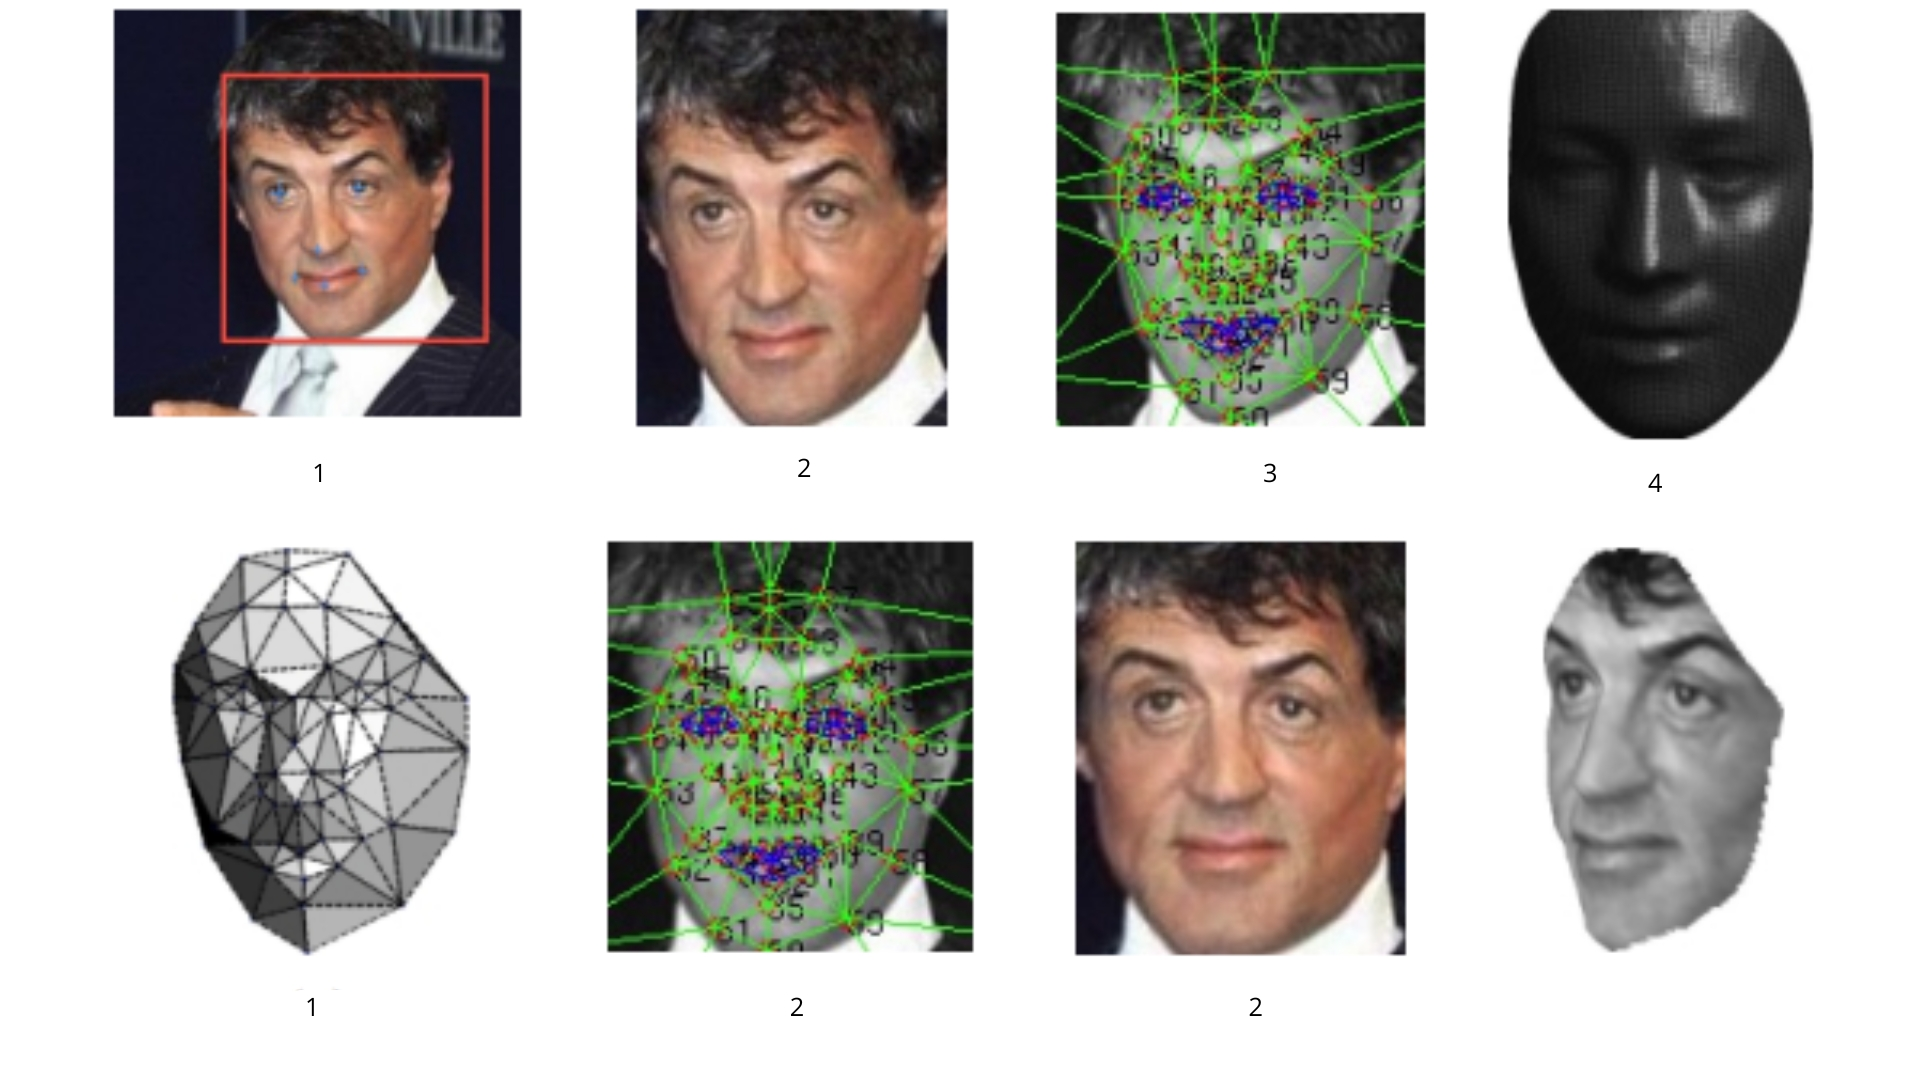
\includegraphics[width=1\textwidth]{img/referencial/deepface-face_classification.jpg}
    \label{fig:etapasPipeline} 
    \vspace{0.3em}
    \footnotesize 
    \vspace{0.2em}
    (a)Detecção; (b)Alinhamento 2D; (c)Pontos fiduciais 2D; 
    (d)Modelo 3D de referência; (e)Visibilidade dos triângulos; 
    (f)Pontos 3D induzidos; (g)Imagem final frontalizada. \\
    \vspace{0.2em} 
    \fonte{Adaptado de \cite{Taigman_2014_CVPR}}
\end{figure}

É fundamental diferenciar os dois modos de operação do reconhecimento. Como definido por \citeonline{braga2013sistemas} e \citeonline{Schroff_2015_CVPR}, as tarefas dividem-se em:

\begin{itemize}
    \item \textbf{Identificação (1:N):} Procura uma correspondência ``um-para-muitos'' para responder à pergunta ``Quem é esta pessoa?'', comparando a face capturada com todos os registros na base de dados.
    \item \textbf{Verificação (1:1):} Valida a identidade ``um-para-um'' respondendo à pergunta ``Esta pessoa é o Paciente João?'', comparando a face capturada apenas com o registro biométrico específico dessa identidade.
\end{itemize}

A precisão dessa correspondência biométrica (seja na identificação ou na verificação) depende fundamentalmente de quão bem o sistema consegue distanciar matematicamente rostos diferentes e aproximar rostos da mesma pessoa no espaço vetorial. Essa lógica de otimização da rede neural é obtida através do treinamento por Perda Tripla (\textit{Triplet Loss}), cujo funcionamento está evidenciado na Figura \ref{fig:TripletLoss}.

\begin{figure}[H]
    \centering
    \caption{Diagrama de Perda Tripla (Triplet Loss)}
    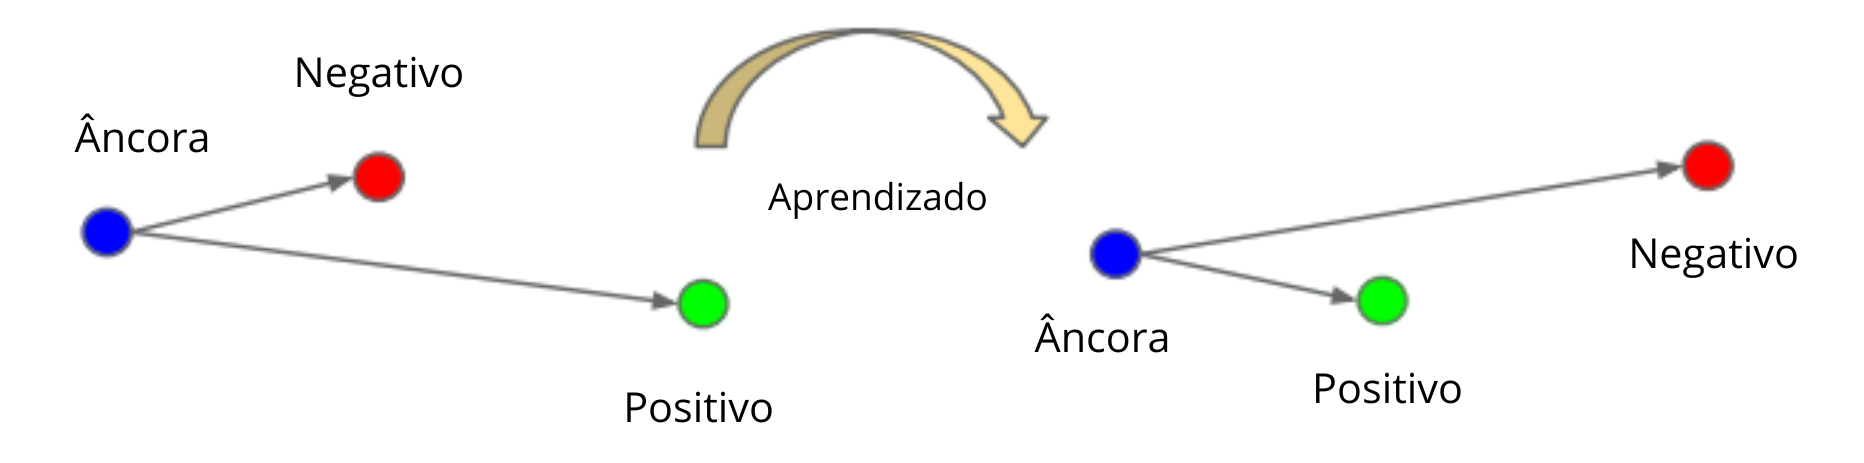
\includegraphics[width=1\textwidth]{img/referencial/FaceNetImage3.png}
    \fonte{Adaptado de \cite{Schroff_2015_CVPR}.}
    \label{fig:TripletLoss}
\end{figure}

Como ilustrado, o modelo aproxima matematicamente as assinaturas da mesma pessoa (Âncora e Positivo) e afasta as de pessoas diferentes (Âncora e Negativo). Consequentemente, quanto menor a distância entre dois \textit{embeddings}, maior a certeza de que pertencem à mesma identidade.

\subsection{EVOLUÇÃO HISTÓRICA: DE ABORDAGENS CLÁSSICAS A REDES NEURAIS}
\label{subsec:abordagens-classicas}

A evolução técnica da visão computacional reflete uma transição significativa nos métodos de extração de características. Inicialmente, o estado da arte era dominado por métodos baseados em características artesanais, como o classificador em cascata proposto por \citeonline{990517}, que utilizava características \textit{Haar-like} para identificar padrões claros e escuros no rosto durante a etapa de detecção, como evidenciado na Figura \ref{fig:Haar-caracteristicas}.

\begin{figure}[H]
    \centering
    \caption{Representação de características do tipo \textit{Haar} utilizadas na detecção facial}
    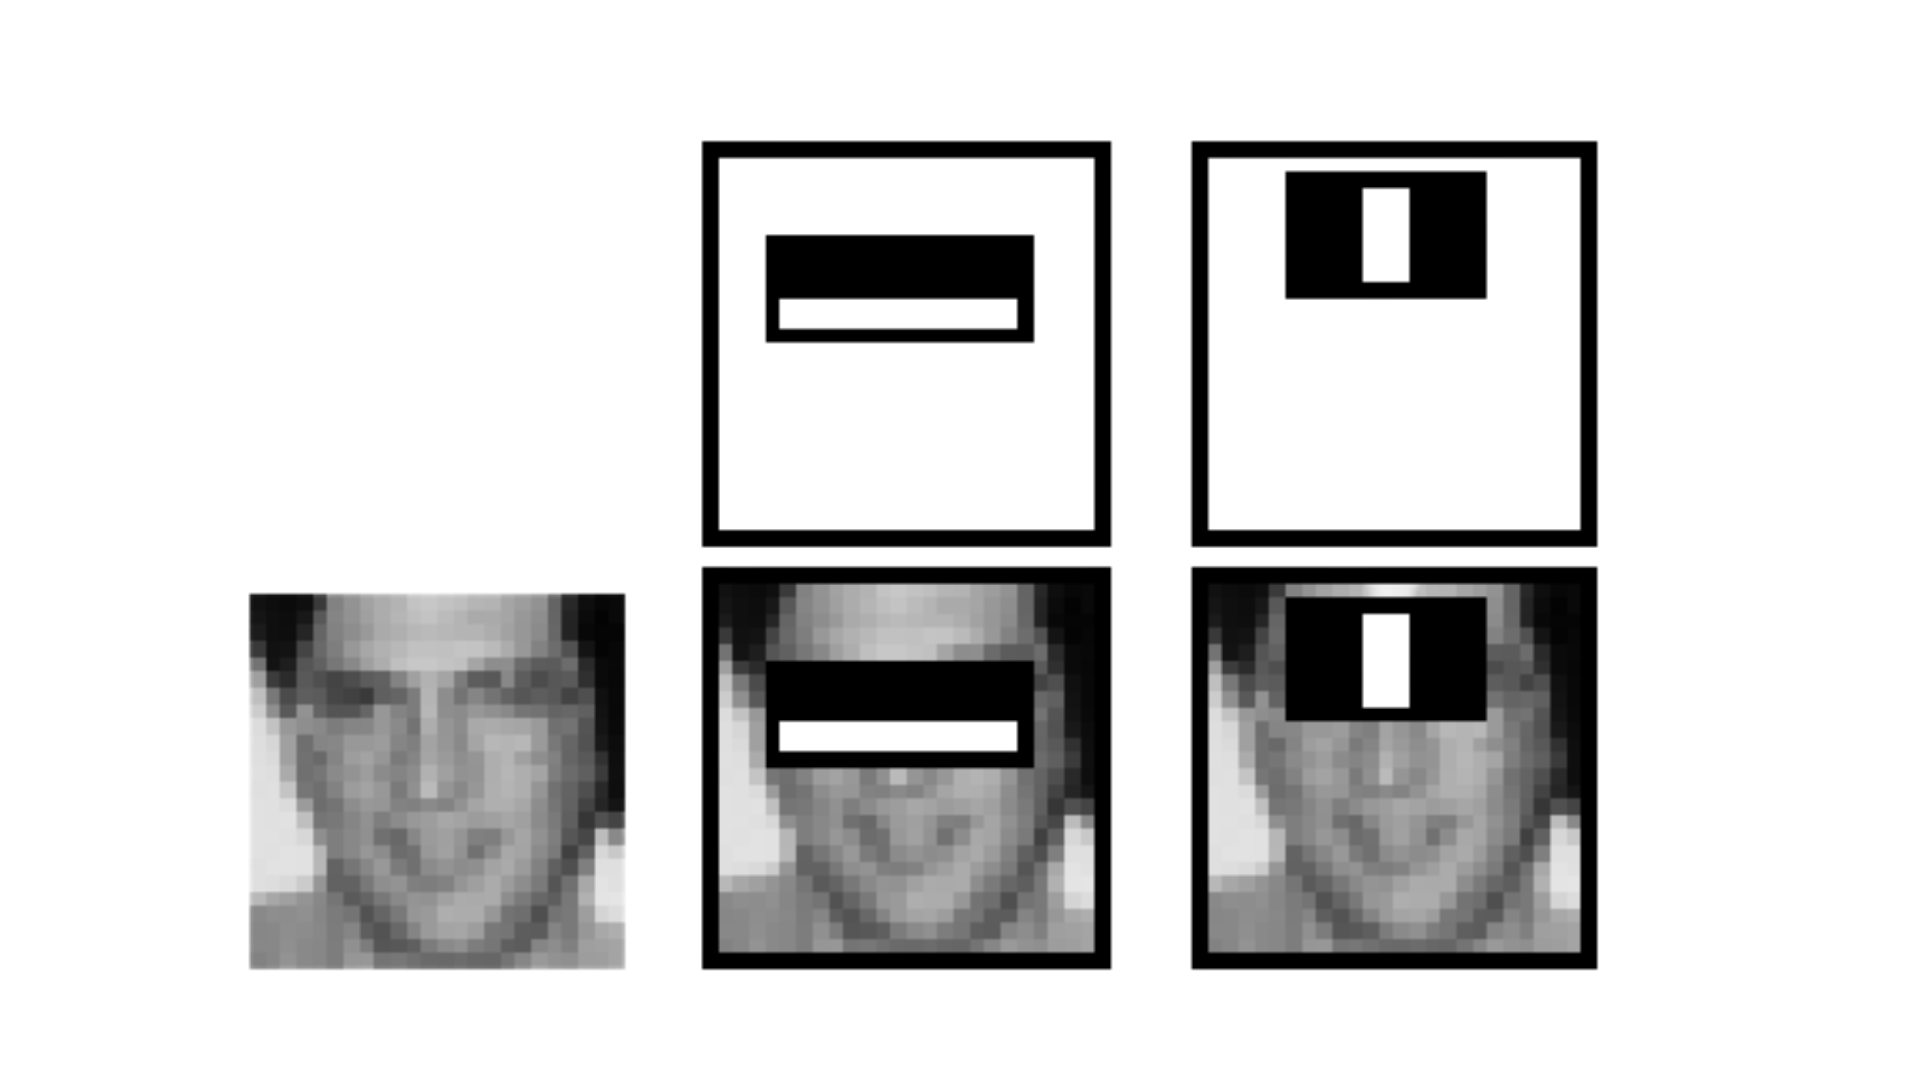
\includegraphics[width=1\textwidth]{img/referencial/person-black_detectation-Viola.png}
    \fonte{Adaptado de \cite{990517}.}
    \label{fig:Haar-caracteristicas}
\end{figure}

Para a etapa de reconhecimento propriamente dita, uma das abordagens pioneiras foi a de \textit{Eigenfaces}, proposta por \cite{10.1162/jocn.1991.3.1.71}, que tratava o reconhecimento facial como um problema intrinsecamente bidimensional (2D). Ou seja, em vez de tentar localizar e medir características individuais de forma isolada (como a distância entre os olhos ou o formato do nariz) — uma tarefa computacionalmente frágil —, a abordagem \textit{Eigenface} analisa a imagem facial como um todo.

O método funciona encontrando os ``componentes principais'' de um grande conjunto de imagens faciais de treino. Estes componentes são vetores que capturam as variações mais significativas entre os rostos. Um novo rosto a ser reconhecido é, então, projetado neste ``espaço facial'' e representado como uma soma ponderada destas \textit{eigenfaces}. A classificação é realizada comparando este vetor de pesos com os vetores de indivíduos conhecidos armazenados na base de dados \cite{10.1162/jocn.1991.3.1.71}. A Figura \ref{fig:projecaoEspacoFinal} ilustra a diferença entre a captura original e a sua projeção reconstruída.

\begin{figure}[H]
    \centering
    \caption{Imagem original e sua projeção no ``espaço facial'' respectivamente.}
    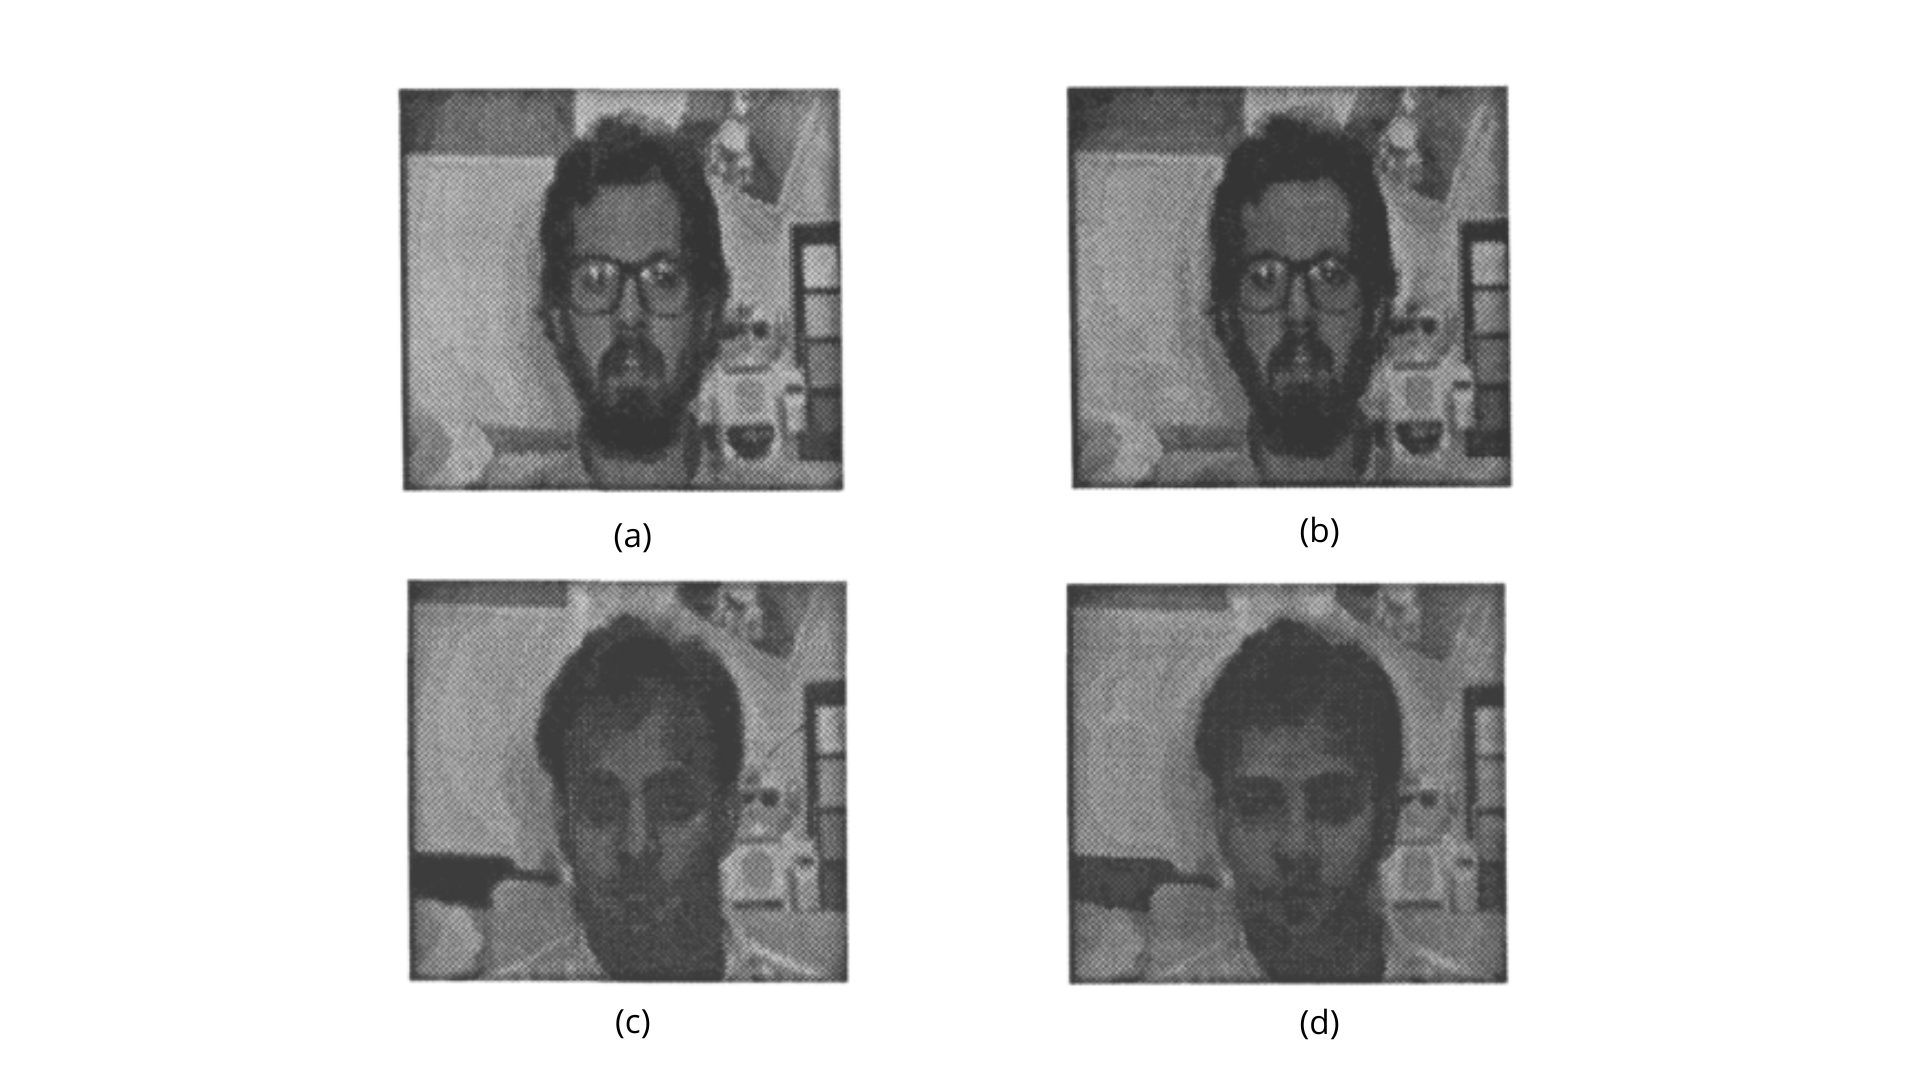
\includegraphics[width=1\textwidth]{img/referencial/EigenfacesImage3.png}
    \label{fig:projecaoEspacoFinal}
    \vspace{0.3em}
    (a) e (c) Imagens originais; (b) e (d) Projeções reconstruídas no ``espaço facial''.
    \\
    \vspace{0.3em}
    \fonte{Adaptado de \cite{10.1162/jocn.1991.3.1.71}.}
\end{figure}

Embora eficientes para a época e fundamentais para provar a viabilidade do reconhecimento facial holístico, esses métodos clássicos apresentavam alta sensibilidade a variações de iluminação, oclusão, escala e pose, como exposto por \citeonline{10.1162/jocn.1991.3.1.71}. Isso ocorre porque, ao dependerem de uma análise estatística da variância dos pixels, qualquer mudança drástica no ambiente físico degrada severamente a precisão do sistema.

Diante dessas limitações em cenários não controlados, a área evoluiu em direção a métodos capazes de aprender representações faciais de forma autônoma. Essa mudança de paradigma consolidou-se com o advento do \textit{deep learning}, em que algoritmos baseados em Redes Neurais Convolucionais (CNNs) superaram a performance humana em diversas métricas de validação, oferecendo uma robustez sem precedentes contra variações de pose e luminosidade \cite{Taigman_2014_CVPR,Schroff_2015_CVPR}.

\subsection{A REVOLUÇÃO DO DEEP LEARNING NO RECONHECIMENTO FACIAL}
\label{subsec:evolucao-historica}

A verdadeira revolução no reconhecimento facial ocorreu com a mudança de paradigma introduzida pelo Aprendizado Profundo (\textit{deep learning}). Em contraste com as abordagens clássicas, que dependiam de características artesanais (\textit{handcrafted}) ou de transformações estatísticas lineares globais sobre a matriz de \textit{pixels}, as Redes Neurais Convolucionais (\textit{CNNs}) — um subtipo especializado das Redes Neurais Profundas (\textit{DNNs}) — possuem a capacidade de aprender representações matemáticas ideais de forma totalmente autônoma a partir de volumes massivos de dados. De acordo com uma revisão sistemática conduzida por \citeonline{soares2025controle}, as \textit{CNNs} consolidaram-se como a técnica de Inteligência Artificial mais empregada no desenvolvimento de sistemas modernos de controle de acesso, representando 54,17\% dos estudos documentados.

Esse sucesso analítico deve-se à arquitetura hierárquica das redes convolucionais. Nas camadas iniciais da rede, os filtros matemáticos extraem características visuais de baixo nível, tais como bordas, texturas e transições de iluminação. À medida que a informação propaga-se pelas camadas intermediárias e profundas, o modelo combina esses elementos primitivos para construir estruturas complexas e invariantes, como o formato geométrico dos olhos, a curvatura do nariz e o contorno mandibular, culminando na representação holística da face humana.

O marco inicial dessa evolução foi o sistema \textit{DeepFace}, proposto por \citeonline{Taigman_2014_CVPR}, que reduziu drasticamente a margem de erro da disciplina ao aproximar-se do nível de acurácia humana. O \textit{DeepFace} demonstrou a eficácia de uma rede neural de nove camadas treinada com mais de 4 milhões de imagens, evidenciando que o aprendizado profundo permite extrair generalizações robustas o suficiente para ignorar ruídos externos de pose e ambiente físico.

Posteriormente, \citeonline{Schroff_2015_CVPR} aperfeiçoaram esse conceito com a introdução do sistema \textit{FaceNet}. A grande inovação deste estudo foi eliminar a necessidade de camadas de classificação pesadas no final da rede, substituindo-as por um mapeamento direto das imagens faciais para um espaço Euclidiano compacto de alta dimensionalidade. A saída gerada por essa arquitetura é denominada \textit{embedding}, que é um vetor de características altamente eficiente.

O \textit{embedding} consiste em um vetor numérico denso (tipicamente composto por 128 ou 512 dimensões \textit{float}) que funciona como uma verdadeira assinatura digital única e invariante do rosto. Dentro desse espaço vetorial real de dimensão finita, a proximidade geométrica reflete a similaridade de identidade: rostos pertencentes ao mesmo indivíduo são projetados em coordenadas próximas (gerando uma distância Euclidiana reduzida), ao passo que faces de indivíduos distintos são mapeadas para pontos distantes no espaço. A Figura \ref{fig:Illuminationandposeinvariance} exemplifica esse comportamento por meio de pares reais de imagens e suas respectivas distâncias no espaço de embedding: quanto mais baixo o valor, maior a probabilidade de pertencerem à mesma identidade.

\begin{figure}[H]
    \centering
    \caption{Exemplos de pares de imagens e suas distâncias no espaço de \textit{embedding}}
    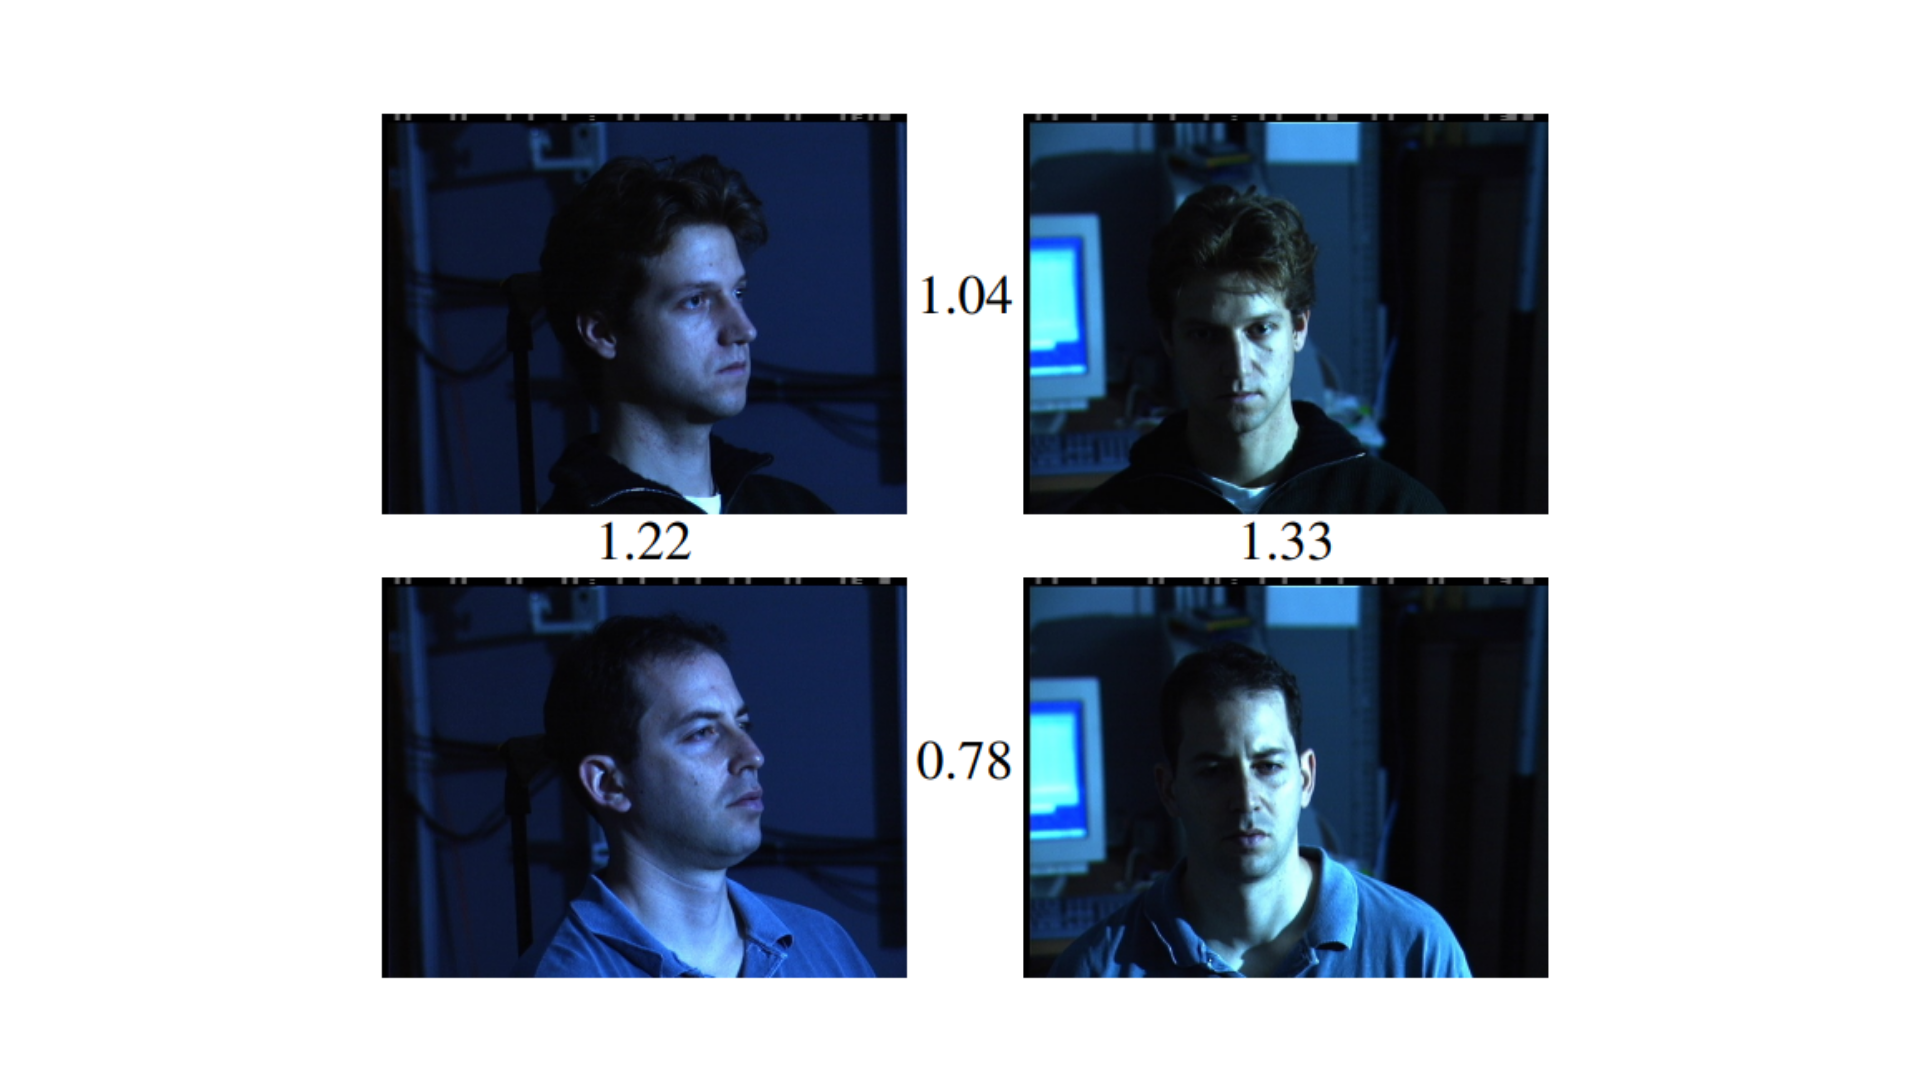
\includegraphics[width=1\textwidth]{img/referencial/Illumination and Pose invariance.png}
    \label{fig:Illuminationandposeinvariance}
    \fonte{Adaptado de \cite{Schroff_2015_CVPR}.}
\end{figure}

Essa estruturação lógica viabiliza a execução de rotinas computacionais extremamente rápidas no dispositivo de borda. Em vez de o \textit{hardware} processar e comparar matrizes complexas de pixels texturizados em tempo real, a tarefa de Identificação (1:N) reduz-se ao cálculo do produto interno e da distância matemática entre vetores compactos de características: o \textit{embedding} extraído da câmera no balcão é rapidamente comparado contra o conjunto de \textit{embeddings} previamente homologados no cadastro de pacientes.


Atualmente, \textit{frameworks} consolidados de visão computacional de código aberto, como o \textit{OpenCV} e bibliotecas avançadas de aprendizado profundo (\textit{Dlib} e \textit{MediaPipe}), encapsulam essas arquiteturas de redes neurais profundas pré-treinadas. A capacidade de extrair e comparar assinaturas digitais de apenas 128 \textit{bytes} com alta eficiência matemática é o pilar que permite que o artefato tecnológico desenvolvido neste trabalho execute a inferência biométrica local de forma instantânea, contornando limitações severas de latência de rede e tornando viável a sua implementação em computadores de placa única de baixo consumo energético e desempenho.

\subsection{DESIGN SCIENCE RESEARCH COMO ABORDAGEM METODOLÓGICA}
\label{subsec:dsr-teorico}

Diferentemente das pesquisas de natureza explicativa, cujo propósito é compreender ou prever fenômenos já existentes, a \textit{Design Science Research} (DSR) situa-se no campo das ciências de projeto: seu objeto não é apenas descrever a realidade, mas produzi-la, por meio da concepção de artefatos capazes de solucionar problemas organizacionais concretos. Consoante \citeonline{hevner2004design}, essa distinção é o que confere à DSR seu caráter singular dentro dos Sistemas de Informação, uma vez que o rigor científico da pesquisa não decorre da observação passiva de um fenômeno, mas da construção deliberada de uma solução e da avaliação sistemática de sua capacidade de resolver o problema que a motivou.

Para operacionalizar essa lógica de forma reprodutível, \citeonline{peffers2007design} sistematizaram a DSR em um processo estruturado de seis atividades, alinhando-se às diretrizes conceituais propostas por \citeonline{hevner2004design} a um roteiro prático que pesquisadores de diferentes áreas passaram a adotar como referência metodológica. Essa contribuição foi decisiva para a popularização da DSR fora do domínio estritamente acadêmico de sistemas de informação, alcançando também pesquisas aplicadas em engenharia de \textit{software} e computação, como é o caso do presente trabalho.

Em um refinamento posterior dessa base conceitual, \citeonline{hevner2010design} propõe que toda pesquisa em DSR deve articular-se em torno de três ciclos interdependentes. O Ciclo de Relevância conecta o ambiente de aplicação — no caso deste trabalho, a recepção das clínicas de saúde e suas demandas reais de segurança e agilidade — às atividades de projeto, fornecendo os requisitos que o artefato precisa atender e os critérios pelos quais sua avaliação será julgada satisfatória. O Ciclo de Rigor, por sua vez, ancora o desenvolvimento na base de conhecimento científico já consolidada, isto é, nas teorias, métodos e resultados de pesquisas anteriores sobre visão computacional e reconhecimento facial discutidos nas seções precedentes, evitando que o artefato seja concebido de forma alheia ao que já se sabe sobre o problema. Por fim, o Ciclo de Projeto (\textit{Design Cycle}) corresponde ao núcleo iterativo da pesquisa, no qual o artefato é construído, testado e refinado em ciclos sucessivos até que atenda aos requisitos definidos pelo Ciclo de Relevância.

É justamente essa articulação entre relevância prática, embasamento teórico e construção iterativa que diferencia a DSR de uma abordagem de desenvolvimento de \textit{software} convencional: o produto final não é apenas um sistema funcional, mas também conhecimento científico generalizável sobre como problemas semelhantes podem ser solucionados. A aplicação prática dessa lógica ao contexto do totem de reconhecimento facial proposto neste trabalho, incluindo a operacionalização das seis atividades de \citeonline{peffers2007design}, é detalhada na Seção \ref{sec:metodologia}.

\subsection{CONTROLE DE ACESSO E ACEITAÇÃO NA SAÚDE}
\label{subsec:controle-acesso}

A aplicação da visão computacional e do reconhecimento facial transcende o mero exercício acadêmico, apresentando-se como uma solução pragmática para problemas operacionais críticos. No setor da saúde, a gestão do fluxo de pessoas e o controle de acessos nas recepções são desafios diários. Os sistemas de credenciamento tradicionais, predominantemente dependentes de verificação humana e documentos físicos, demonstram ser lentos e suscetíveis a falhas de caráter humano, culminando no aumento de filas e no desgaste dos pacientes e colaboradores num ambiente que exige acolhimento ágil \cite{10.1371/journal.pone.0257923}.

Neste cenário, as Tecnologias de Reconhecimento Facial (\textit{FRTs - Facial Recognition Technologies}) têm sido progressivamente incorporadas aos protocolos hospitalares e clínicos. As suas aplicações práticas vão desde a otimização do \textit{check-in} de pacientes de forma estritamente sem contato, até à validação inequívoca da identidade para garantir a correspondência exata com o registro médico eletrônico, mitigando o risco de erros médicos.

A viabilidade da adoção de tecnologias biométricas nestes ambientes está, no entanto, intrinsecamente ligada à percepção e aceitação do público. Num amplo levantamento conduzido por \citeonline{10.1371/journal.pone.0257923} sobre as perspectivas dos usuários em contextos clínicos, observou-se que a maioria dos indivíduos considera aceitável a utilização de \textit{FRTs} desde que o propósito seja delimitado e traga benefícios diretos para a segurança do paciente.

Conforme evidenciado pelo estudo, 65,9\% apoiam o uso do reconhecimento facial quando a finalidade é verificar a identidade de pacientes para evitar erros médicos, e 63,4\% aceitam a tecnologia para identificar pacientes que não respondem ou se encontram desacompanhados. Em contrapartida, a aceitabilidade decai significativamente para faixas mais baixas (como 58\%) quando o uso sugere o mero cruzamento de dados de saúde para fins mais generalistas. A Figura \ref{fig:grafico-aceitabiliade} ilustra os diferentes níveis de tolerância relatados pela pesquisa.

\begin{figure}[H]
    \centering
    \caption{Gráfico de aceitabilidade de tecnologias de reconhecimento facial em três cenários de saúde.}
    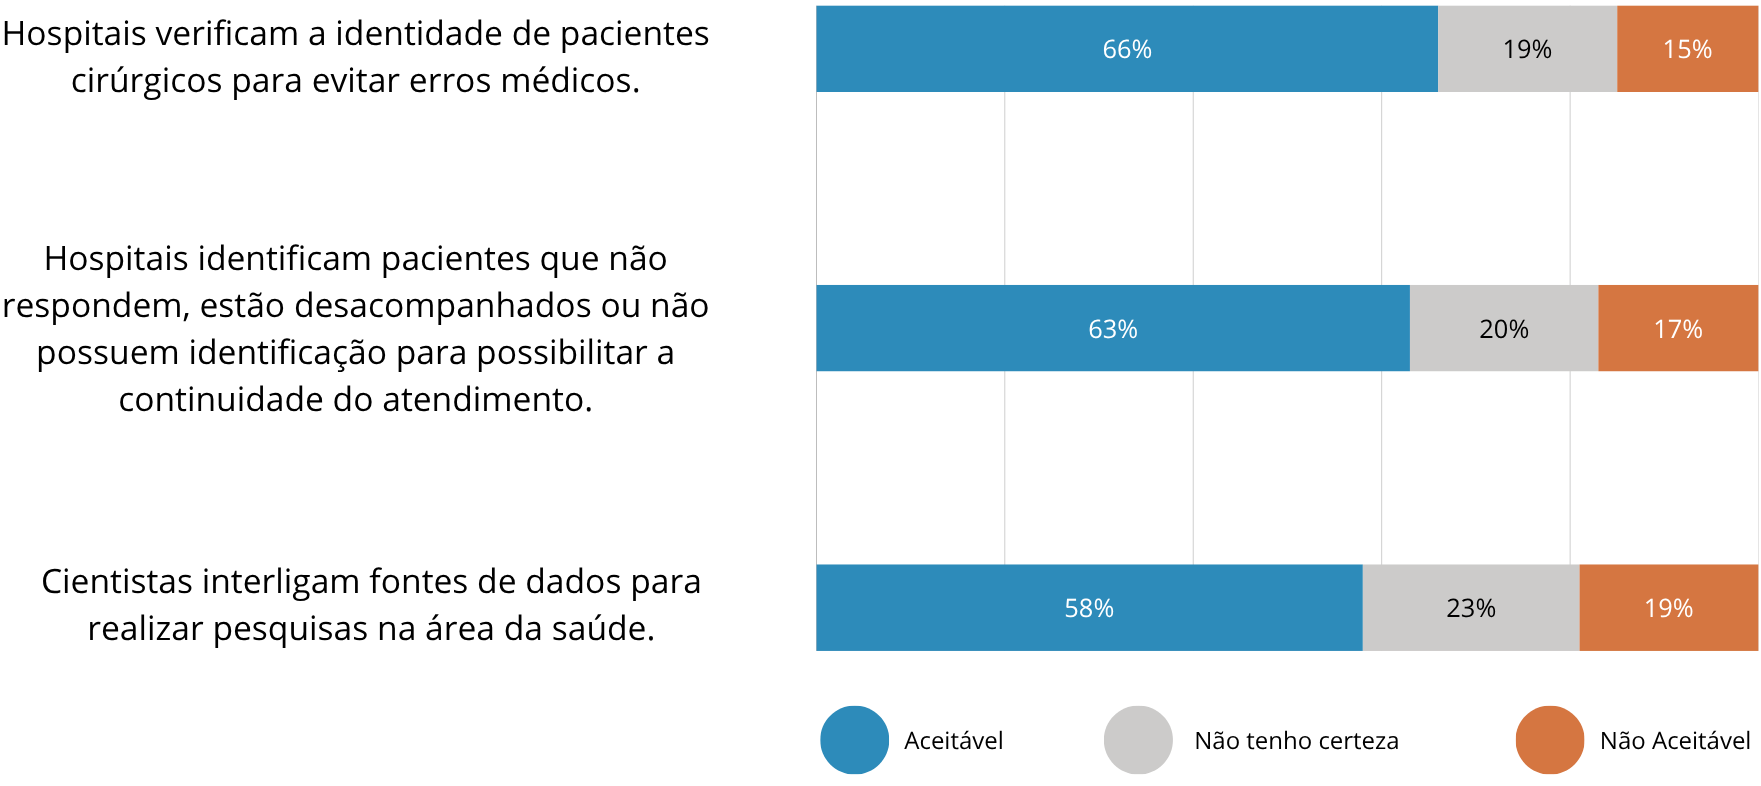
\includegraphics[width=1\textwidth]{img/referencial/AsurveyofImage1.png} 
    \vspace{0.3em}
    \footnotesize 
    \label{fig:grafico-aceitabiliade}
    \fonte{Adaptado de \cite{10.1371/journal.pone.0257923}.}
\end{figure}

Estes dados empíricos validam a premissa de que a substituição de processos manuais no balcão de recepção por um sistema de validação de caráter facial é uma estratégia não apenas viável, mas bem aceita pelo público quando feita com transparência para agilizar e proteger o atendimento. Contudo, as preocupações manifestadas pelos usuários em relação à privacidade dos seus dados (como o envio de imagens faciais para servidores remotos) exigem que a arquitetura destes sistemas seja projetada com rigor extremo.

É precisamente para suprir esta necessidade estrita de privacidade e latência que a solução arquitetural adotada neste trabalho abandona o processamento em nuvem a favor do paradigma da Computação de Borda, temática abordada na seção a seguir.

\subsection{ESTUDOS RELACIONADOS E SÍNTESE DA LITERATURA}
\label{subsec:estudos-relacionados}

Para consolidar o panorama tecnológico e identificar as tendências consolidadas no desenvolvimento de sistemas de controle de acesso automatizados, faz-se necessário analisar como a literatura científica recente aborda a convergência entre Inteligência Artificial e Visão Computacional. Nesse cenário, mapear os algoritmos mais utilizados e as arquiteturas de \textit{software} prediletas por pesquisadores da área fornece o embasamento necessário para validar as escolhas de projeto deste trabalho.

Um indicador analítico de extrema relevância para esta pesquisa é o mapeamento estatístico conduzido por \citeonline{soares2025controle}, que realizou uma revisão sistemática da literatura focada estritamente em sistemas de controle de acesso baseados em reconhecimento facial. O estudo estatístico quantificou quais técnicas de Inteligência Artificial e quais abordagens algorítmicas de Visão Computacional apresentam maior recorrência e eficácia no cenário acadêmico e de desenvolvimento atual.

Os dados sintetizados por \citeonline{soares2025controle} apontam que as Redes Neurais Convolucionais (\textit{CNNs}) lideram isoladamente como a técnica de Inteligência Artificial mais empregada na disciplina, estando presentes em 54,17\% dos sistemas mapeados. No que tange aos algoritmos específicos para a etapa de detecção e processamento de faces, o Classificador em Cascata de \textit{Haar} (\textit{HCC — Haar Cascade Classifier}) mantém uma presença expressiva de 31,25\% devido à sua leveza computacional histórica, seguido por abordagens baseadas em histogramas locais (\textit{LBPH}) e ferramentas de extração avançadas, como a biblioteca \textit{Dlib}. O \autoref{qua:comparacao_ia} apresenta detalhadamente a distribuição e classificação dessas tecnologias segundo a literatura.

\begin{quadro}[htbp]
    \centering
    \caption{Comparação de Técnicas de IA e Algoritmos na Literatura}
    \label{qua:comparacao_ia}
    \small
    \begin{tabularx}{\textwidth}{|>{\centering\arraybackslash}p{1.4cm}|>{\raggedright\arraybackslash}X|>{\raggedright\arraybackslash}X|}
        \hline
        \textbf{Posição} & \textbf{Técnica de IA (\%)} & \textbf{Abordagem Algorítmica (\%)} \\
        \hline
        1º & Redes Neurais Convolucionais — CNN (54,17\%) & Classificador em Cascata de \textit{Haar} — HCC (31,25\%) \\
        \hline
        2º & Redes Neurais Tradicionais — RN (29,17\%) & \textit{Local Binary Patterns Histograms} — LBPH (12,50\%) \\
        \hline
        3º & \textit{Deep Learning} Geral — DL (27,08\%) & Biblioteca de Visão Computacional — Dlib (10,42\%) \\
        \hline
    \end{tabularx}
    \fonte{Adaptado de \citeonline{soares2025controle}.}
    % \fonte{Adaptado de Soares et al. (2025).}
\end{quadro}

A análise dos dados expostos no \autoref{qua:comparacao_ia} mostra que a combinação de Redes Neurais Convolucionais com bibliotecas consagradas de visão computacional constitui o estado da arte para o desenvolvimento de sistemas de segurança biométrica. É exatamente com base neste sólido alicerce teórico — que abrange desde o processamento matemático das imagens até a alta aceitabilidade do público em ambientes clínicos — que as diretrizes técnicas deste trabalho foram definidas.

\section{METODOLOGIA}
\label{sec:metodologia}

 Este capítulo detalha o percurso metodológico adotado para a concepção, desenvolvimento e validação do artefato tecnológico proposto. A pesquisa fundamenta-se na metodologia \textit{DSR}, que, consoante a \citeonline{hevner2010design}, se destaca no campo dos Sistemas de Informação por focar na resolução de problemas práticos através da construção de um artefato tecnológico, gerando também novo conhecimento científico. Para melhor compreensão visual do fluxo metodológico, o processo adotado encontra-se esquematizado na \autoref{fig:etapas-desenvolvimento-dsr}.

\begin{figure}[H]
    \centering
    \caption{Etapas de Metodologia \textit{DSR}}
    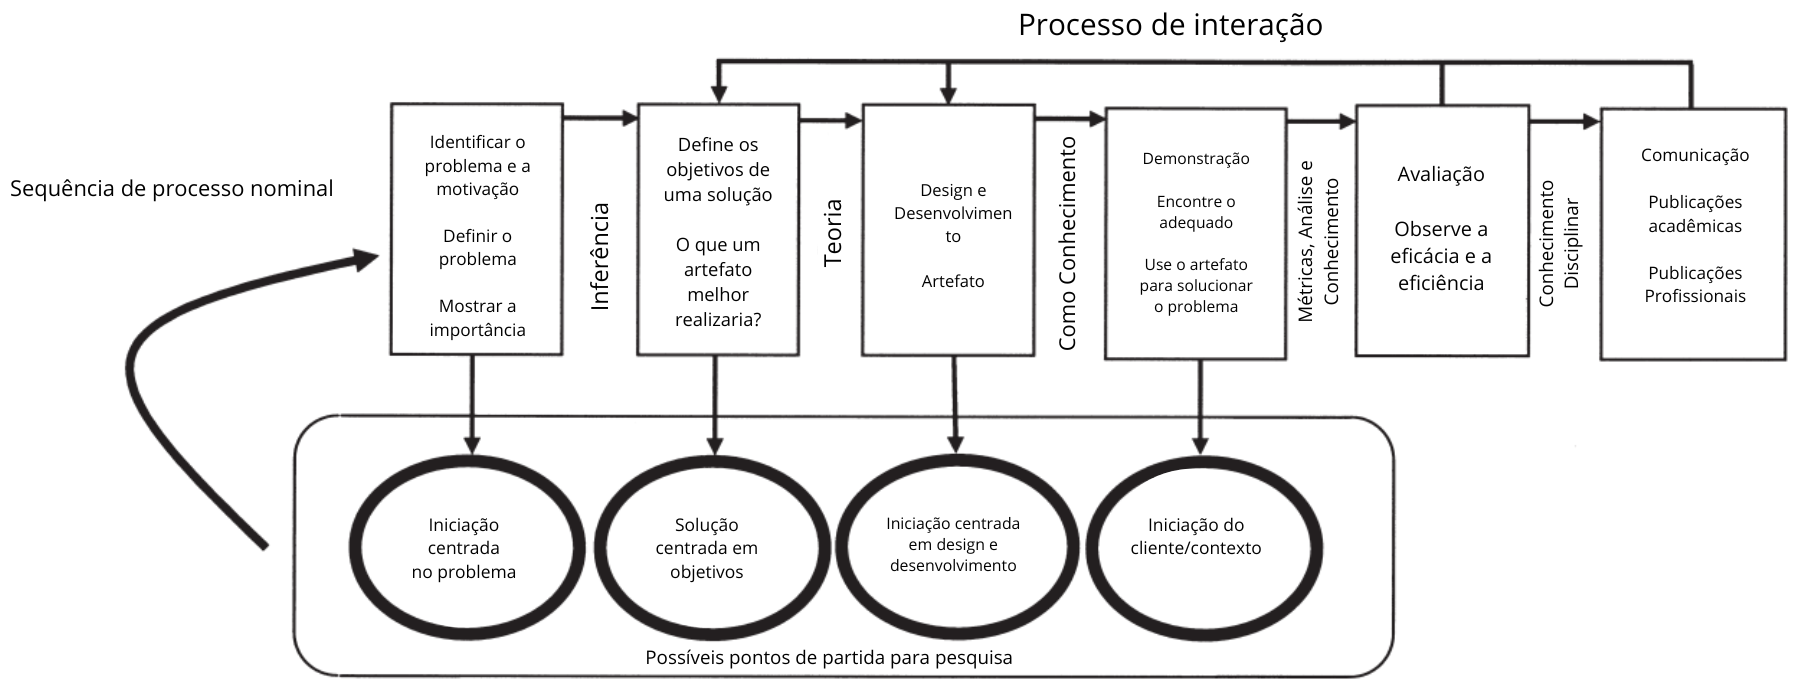
\includegraphics[width=1\textwidth]{img/referencial/etapasDesenvolvimentoDSR.png} 
    \vspace{0.3em}
    \footnotesize 
    \label{fig:etapas-desenvolvimento-dsr}
    \fonte{Traduzido de \cite{peffers2007design}.}
\end{figure}

Este trabalho segue o modelo de processo composto de seis etapas proposto por \citeonline{peffers2007design}. As seções a seguir descrevem como cada uma dessas etapas foi aplicada à realidade das clínicas de saúde da região para a validação do totem de reconhecimento facial, que será melhor abordado na Subseção  \ref{subsec:estapas-dsr}.

\subsection{CARACTERIZAÇÃO DA PESQUISA}
\label{subsec:caracterizacao}

Do ponto de vista da sua natureza, a pesquisa classifica-se como aplicada, pois busca solucionar um problema prático específico: a lentidão e o gargalo no processo de credenciamento em instituições de saúde. Quanto aos objetivos, caracteriza-se como exploratória, visando testar a viabilidade e aprimorar a implementação de uma arquitetura inovadora de Computação de Borda no cenário clínico local, alinhando-se à abordagem de desenvolvimento de artefatos da \textit{DSR} \citeonline{gil2019}.

A abordagem adotada é quantitativa, uma vez que a validação do artefato exige a mensuração, comparação matemática e análise estatística de variáveis de desempenho (tempo de \textit{check-in} manual contra automatizado) para a testagem das hipóteses \citeonline{creswell2018}.

Por fim, em relação aos procedimentos técnicos, delineia-se como pesquisa experimental com estudo de campo. Essa classificação, segundo \citeonline{marconi2017}, justifica a instanciação, o controle e a cronometragem objetiva do protótipo biométrico no ambiente real das clínicas, cumprindo rigorosamente as etapas de Demonstração e Avaliação exigidas pela metodologia \textit{Design Science Research}.

\subsection{POPULAÇÃO E AMOSTRA}
\label{subsec:populacao-amostra}

A população desta pesquisa é constituída pelas instituições de assistência à saúde (clínicas e consultórios médicos) privadas e filantrópicas localizadas no município de Floriano-PI, bem como pelo fluxo total de pacientes que demandam atendimento diário de credenciamento e recepção nesses estabelecimentos.

Para a definição da amostra, foi utilizada a técnica de amostragem não probabilística por conveniência, que, segundo \citeonline{hair2019}, é adequada quando o investigador seleciona os elementos amostrais com base na sua disponibilidade, proximidade e acessibilidade física ou institucional, sendo uma abordagem amplamente adotada em investigações de caráter exploratório e experimental onde a amostragem probabilística estrita se torna operacionalmente inviável devido a restrições de tempo, custos ou barreiras de acesso a dados sigilosos.

O tamanho da amostra foi determinado considerando critérios de viabilidade técnica e relevância prática para o mapeamento de processos e validação do artefato, resultando na seleção de três clínicas de saúde de médio porte atuantes no município. A amostragem englobou a análise do fluxo de atendimento de balcão e a cronometragem dos tempos operacionais de registro de pacientes divididos entre uma clínica oftalmológica, uma clínica odontológica e uma instituição de atendimento multidisciplinar, totalizando 14 atendimentos de credenciamento cronometrados (4 na clínica oftalmológica, 5 na clínica odontológica e 5 na instituição multidisciplinar), número compatível com o caráter exploratório desta etapa de diagnóstico e estabelecendo assim a base de dados empírica necessária para avaliar o impacto do Artefato Tecnológico desenvolvido.

\subsection{COLETA DE DADOS}
\label{subsec:coleta-dados}

A coleta de dados foi estruturada em duas frentes distintas — o diagnóstico do cenário atual e a aferição do artefato tecnológico —, utilizando instrumentos específicos que permitiram obter informações quantitativas e operacionais essenciais para a etapa de Avaliação da metodologia. Os instrumentos escolhidos para esta investigação foram:

\begin{itemize}
    \item \textbf{Formulário de Mapeamento de Processos:} Aplicado junto à gestão e aos atendentes das três instituições de saúde para levantar informações sobre o fluxo de atendimento no balcão, totalizando 4 respondentes (um na clínica oftalmológica, um na clínica odontológica e dois na instituição multidisciplinar). A utilização deste instrumento justifica-se por fornecer o diagnóstico dos estrangulamentos do processo manual, permitindo identificar que a lentidão decorre fundamentalmente da etapa de ``cadastro'' e das falhas na apresentação de documentos físicos por parte dos pacientes.
    \item \textbf{Observação Direta e Cronometragem em campo:} Utilizada para aferir o tempo cronometrado em minutos e segundos que cada paciente demora na fila de recepção. Este procedimento justifica-se pela necessidade estrita de estabelecer uma \textit{baseline} (linha de base) verdadeira e quantitativa do método tradicional (como as médias de 6 a quase 9 minutos documentadas), garantindo que os dados refletem o ambiente natural das clínicas sem o viés da percepção subjetiva.
    \item \textbf{Testes de Desempenho Computacional (\textit{Logs} do Sistema):} Ferramenta de recolhimento de dados implementada no próprio código-fonte do \textit{SBC} Labrador durante a fase de Demonstração do totem. Este instrumento justifica-se por ser a única forma de mensurar, com precisão de milissegundos, a variável de Performance da solução tecnológica (o tempo de inferência da rede neural e do cálculo de distância Euclidiana), permitindo assim o contraste direto e matemático contra a \textit{baseline} do processo manual.
\end{itemize}

\subsection{PROCEDIMENTOS METODOLÓGICOS: ETAPAS DA DSR}
\label{subsec:estapas-dsr}

Conforme estabelecido na fundamentação metodológica deste estudo, o percurso operacional para a construção e validação da solução tecnológica segue rigorosamente o modelo de processo nominal da \textit{Design Science Research} proposto por \cite{peffers2007design}.

\subsubsection{Identificação do Problema e Motivação}
\label{subsubsec:problema-motivacao}

A etapa inicial da \textit{DSR} consiste em definir o problema específico e justificar o valor da solução. Através do mapeamento empírico de processos de negócio realizado em clínicas na cidade de Floriano-PI - citados anteriormente -, identificou-se que o credenciamento de pacientes é realizado de forma predominantemente manual. Esse método exige a apresentação de documentos físicos e a interação contínua com atendentes, resultando em tempos médios de espera que variam entre 6 a quase 9 minutos por paciente. A motivação para a intervenção tecnológica nasce da necessidade de mitigar esses gargalos operacionais, transformando um processo demorado e físico em um fluxo digital e sem atrito \cite{peffers2007design}.

\subsubsection{Objetivos da Solução}
\label{subsubsec:objetivos-solução}

A partir do problema diagnosticado, a segunda etapa infere racionalmente os objetivos que o artefato deve atingir \citeonline{peffers2007design}. O objetivo central estabelecido para esta solução foi automatizar e acelerar o controle de acesso de pacientes por meio de um totem de Reconhecimento Facial, visando reduzir o tempo de espera nas filas. É fundamental ressaltar que os dados empíricos coletados nas clínicas para a fundamentação deste estudo foram tratados de forma totalmente anônima, sem a coleta de nomes ou de qualquer informação que identificasse os pacientes ou as instituições. Para garantir a viabilidade técnica e a agilidade operacional do artefato, estipulou-se que o sistema deveria operar sob o paradigma da Computação de Borda, realizando a validação de forma local, \textit{offline} e em tempo real, sem a necessidade de transmitir as imagens capturadas para servidores em nuvem.

\subsubsection{Design e Desenvolvimento}
\label{subsubsec:design-desenvolvimento}

Esta etapa compreende a criação estrutural da solução, definindo rigorosamente a arquitetura de \textit{hardware} e o ecossistema de \textit{software} necessários para materializar os objetivos propostos \citeonline{peffers2007design}. O design do Artefato foi concebido através da integração otimizada de componentes de baixo custo e alta eficiência, divididos em duas camadas principais:

\begin{itemize}
    \item A infraestrutura de \textit{hardware} foi desenhada para operar de forma autônoma na recepção das clínicas, sendo composta por:

    \begin{itemize}
        \item \textbf{\textit{SBC} Labrador (Núcleo de Processamento):} O Computador de Placa Única atua como o ``cérebro'' do sistema, sendo o responsável exclusivo por executar o ambiente \textit{Python}, processar os cálculos matemáticos intensivos das redes neurais e realizar a validação dos vetores faciais de forma totalmente local. A escolha do Labrador, em detrimento de alternativas consolidadas no mercado internacional, como o \textit{Raspberry Pi}, fundamenta-se em fatores estratégicos e operacionais. Por tratar-se de um equipamento de arquitetura nacional, o dispositivo oferece maior disponibilidade e agilidade de aquisição no mercado brasileiro, contornando a volatilidade de preços, a escassez de fornecimento e as altas taxas de importação de componentes estrangeiros. Além de apresentar uma excelente relação de custo-benefício para a prototipagem, a adoção deste \textit{hardware} atua diretamente como um vetor de fomento à tecnologia produzida no país, comprovando que soluções nacionais possuem maturidade estrutural e computacional para suportar o processamento intensivo de Computação de Borda.
        \item \textbf{Sensor de Distância a Laser VL53L0X (Gatilho de Ação):} Componente crítico que monitora continuamente o ambiente com precisão milimétrica. Ao detectar a aproximação física de um paciente a uma distância pré-configurada (80 centímetros), ele envia um sinal de interrupção que ``desperta'' o sistema de captura, tornando a interação 100\% sem contato e otimizando o consumo de energia e desempenho.
        \item \textbf{Módulo de Câmera OV2640:} Acionado pelo gatilho de proximidade, é o sensor ótico encarregado de capturar a imagem do rosto do paciente em tempo real e transmiti-la para o processamento primário.
        \item \textbf{Painel IPS 7P:} Uma tela de 7 polegadas que atua como interface visual, onde o usuário visualiza as instruções de uso, o retorno em tempo real da câmera e os alertas de liberação.
        \item \textbf{CASE 3D:} A estrutura física protetora. Uma carcaça modelada e impressa em 3D, projetada sob medida para acomodar a eletrônica, organizar a fiação e fixar o painel, garantindo um acabamento profissional e ergonômico.

        \begin{figure}[H]
            \centering
            \caption{Arquitetura de \textit{hardware} e componentes estruturais do Artefato.}
            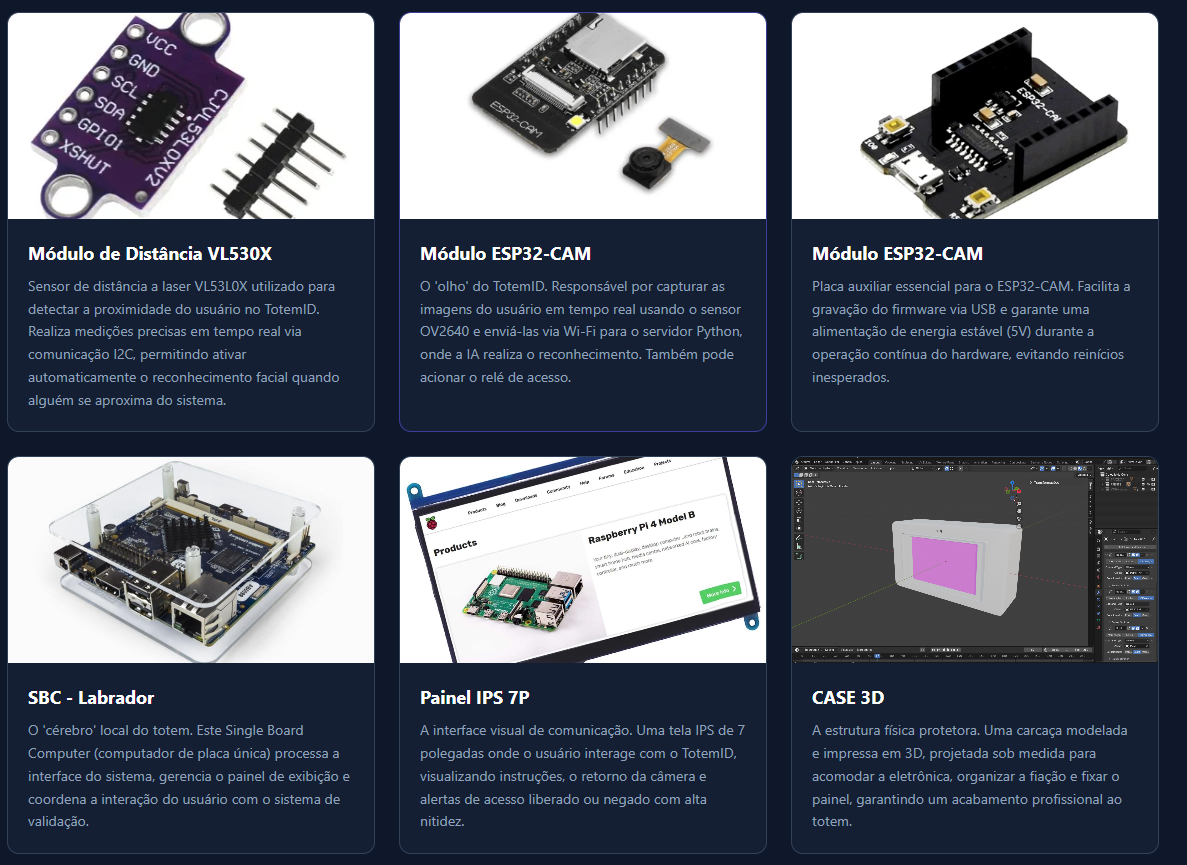
\includegraphics[width=1\textwidth]{img/metodologia/componentes-hardware.png}
            \fonte{Elaborado pelo Autor (2026).}
            \label{fig:componentes-hardware}
        \end{figure}
    \end{itemize}

    \item Da mesma forma, a arquitetura de \textit{Software} e fluxo de integração foi concebida por:

    \begin{itemize}
        \item O pipeline de visão computacional implementado atua em múltiplas fases, apoiando-se em algoritmos nativos da biblioteca \textit{Dlib}. Para a etapa inicial de detecção e localização espacial das faces no quadro capturado, o sistema adota o modelo \textit{HOG} (\textit{Histogram of Oriented Gradients}) em conjunto com um classificador \textit{SVM} (\textit{Support Vector Machine}) linear, assegurando um processamento leve e otimizado diante das restrições de \textit{hardware} do \textit{SBC} Labrador. Na etapa subsequente, a extração das assinaturas biométricas é realizada por meio de uma arquitetura de Rede Neural Residual (\textit{ResNet}) pré-treinada com 29 camadas convolucionais (\textit{dlib\_face\_recognition\_resnet\_model\_v1.dat}). Este modelo projeta as características faciais em um espaço Euclidiano de alta dimensionalidade, gerando um \textit{embedding} denso e invariante de exatas 128 dimensões (128-D) em formato de ponto flutuante. A etapa final de verificação e liberação de acesso baseia-se no cálculo da distância Euclidiana entre o vetor capturado em tempo real e os vetores armazenados na base de dados local (\textit{encodings.pickle)}. Para garantir um elevado nível de segurança e mitigar falsos aceites, estabeleceu-se um limiar (\textit{threshold}) estrito de tolerância máxima de $0,3$ para a distância Euclidiana normalizada entre os vetores. Matematicamente, o sistema processa a liberação apenas se a distância vetorial for menor ou igual a este limite — é este valor bruto de distância, e não o percentual de confiança, que rege a decisão binária de LIBERADO/NEGADO. O percentual de confiança (\textit{confianca\_pct}) reportado nos \textit{logs} é uma métrica auxiliar, derivada da mesma distância por meio de uma normalização não linear voltada à leitura humana dos registros; por isso, autenticações liberadas podem apresentar percentuais de confiança variados (ver Seção \ref{desempenho-computacional}) sem que isso represente qualquer inconsistência no critério de liberação, que permanece sempre regido pelo limiar de distância de $0,3$.
        \item A extração das assinaturas digitais matemáticas (\textit{embeddings}) foi fundamentada em arquiteturas de Redes Neurais Profundas;
        \item A comunicação entre as camadas de \textit{software} (o \textit{SBC} Labrador) e de \textit{hardware} (o OV2640) ocorre de maneira orquestrada: o sistema realiza uma varredura de Identificação (1:N) contra o banco de dados local, otimizado para conter os \textit{embeddings} dos pacientes agendados para o turno. Após o SBC encontrar a correspondência e validar a identidade com sucesso, ele emite um sinal de confirmação visual na tela \textit{IPS}, garantindo um ciclo de inferência seguro e de curtíssima latência.
    \end{itemize}
\end{itemize}

O diagrama que sistematiza a convergência entre os componentes de \textit{hardware} e o \textit{pipeline} de \textit{software} operando no dispositivo de borda encontra-se detalhado na Figura \ref{fig:fluxograma-arquitetura}.

\begin{figure}[H]
    \centering
    \caption{Diagrama de integração do pipeline de reconhecimento facial e resposta periférica.}
    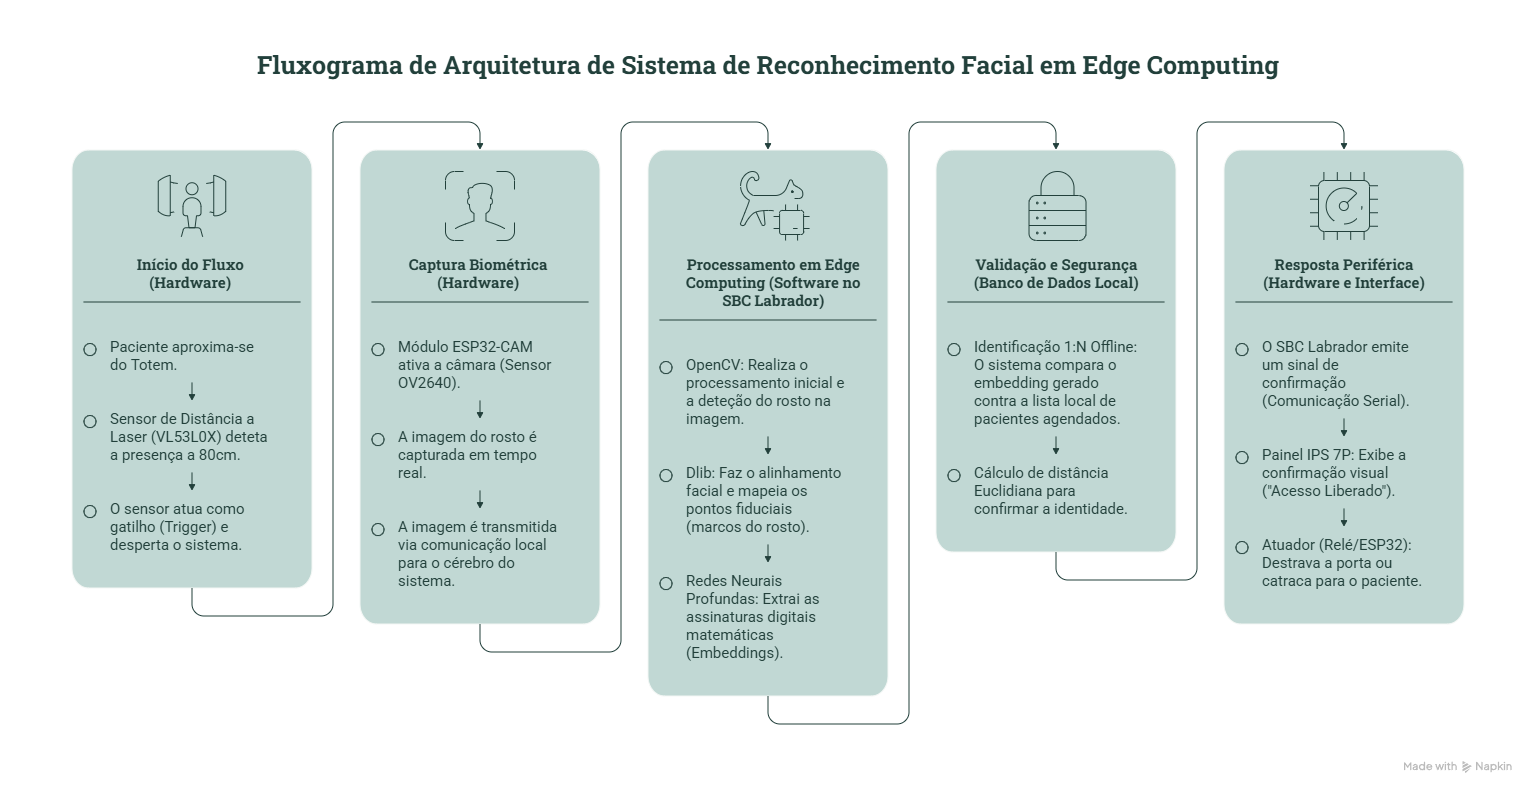
\includegraphics[width=0.9\textwidth]{img/metodologia/fluxograma de arquitetura de sistema de reconhecimento facial.png}
    \fonte{Elaborado pelo Autor (2026).}
    \label{fig:fluxograma-arquitetura}
\end{figure}

\subsubsection{Demonstração}
\label{subsubsec:demonstracao}

A quarta etapa da \textit{DSR} exige a aplicação empírica do artefato para demonstrar sua capacidade de solucionar o problema \citeonline{peffers2007design}. A demonstração operacional deste trabalho ocorreu por meio da instanciação do Artefato Tecnológico (Totem de Reconhecimento Facial) configurado com o ambiente de execução do \textit{SBC} Labrador acoplado ao \textit{hardware} auxiliar. Foram simulados os fluxos de credenciamento em cenário realístico, submetendo o conjunto formado pelo sensor ótico (OV2640) e pelo módulo de distância a laser (VL53L0X) a diferentes aproximações de usuários previamente cadastrados para testar a responsividade do código e a emissão de resposta física. A Figura \ref{fig:reconhecimento-tempo-real} apresenta duas capturas de validação desse reconhecimento em tempo real, evidenciando que o sistema mantém a identificação correta do usuário cadastrado mesmo diante de pequenas variações de aparência, como o uso de boné.

\begin{figure}[H]
    \centering
    \caption{Capturas de validação do reconhecimento facial em tempo real}
    \begin{minipage}{0.48\textwidth}
        \centering
        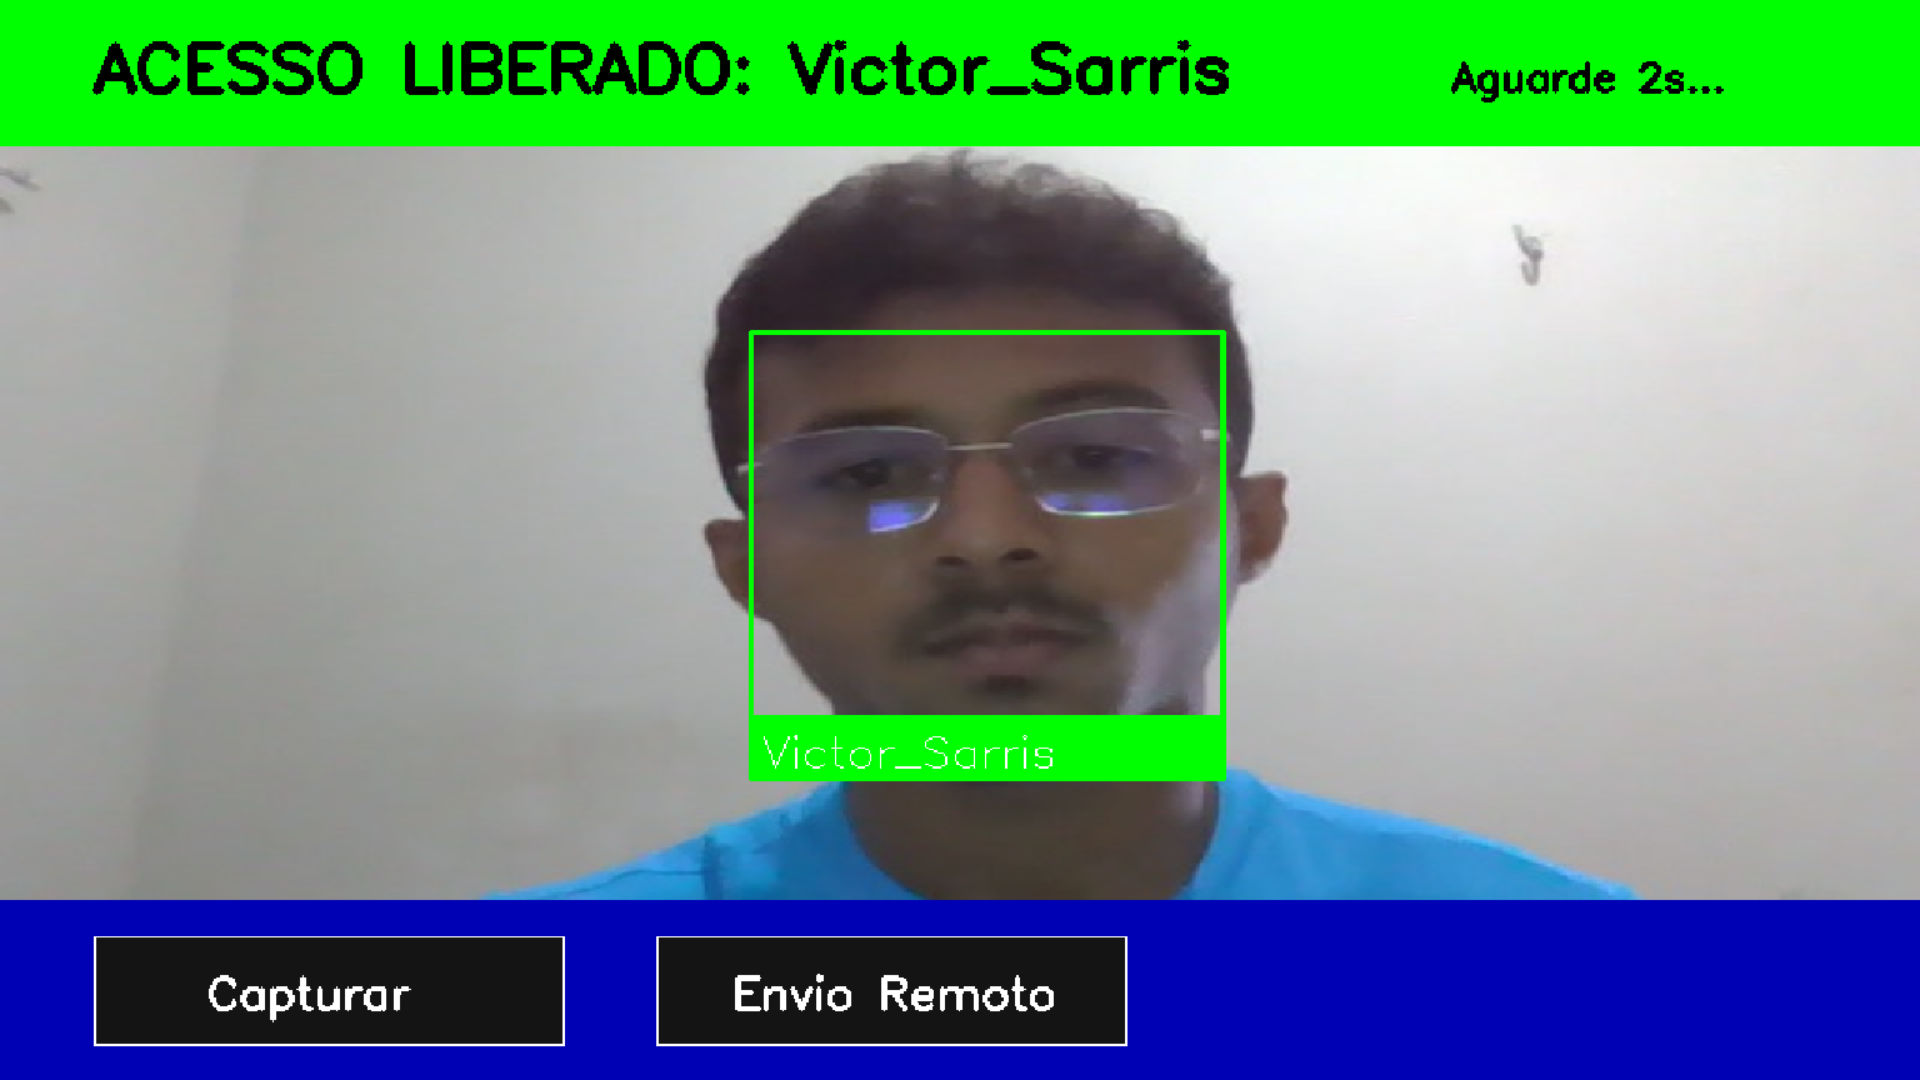
\includegraphics[width=\textwidth]{img/metodologia/reconhecimento1.png}
        \\ (a) Sem boné
    \end{minipage}
    \hfill
    \begin{minipage}{0.48\textwidth}
        \centering
        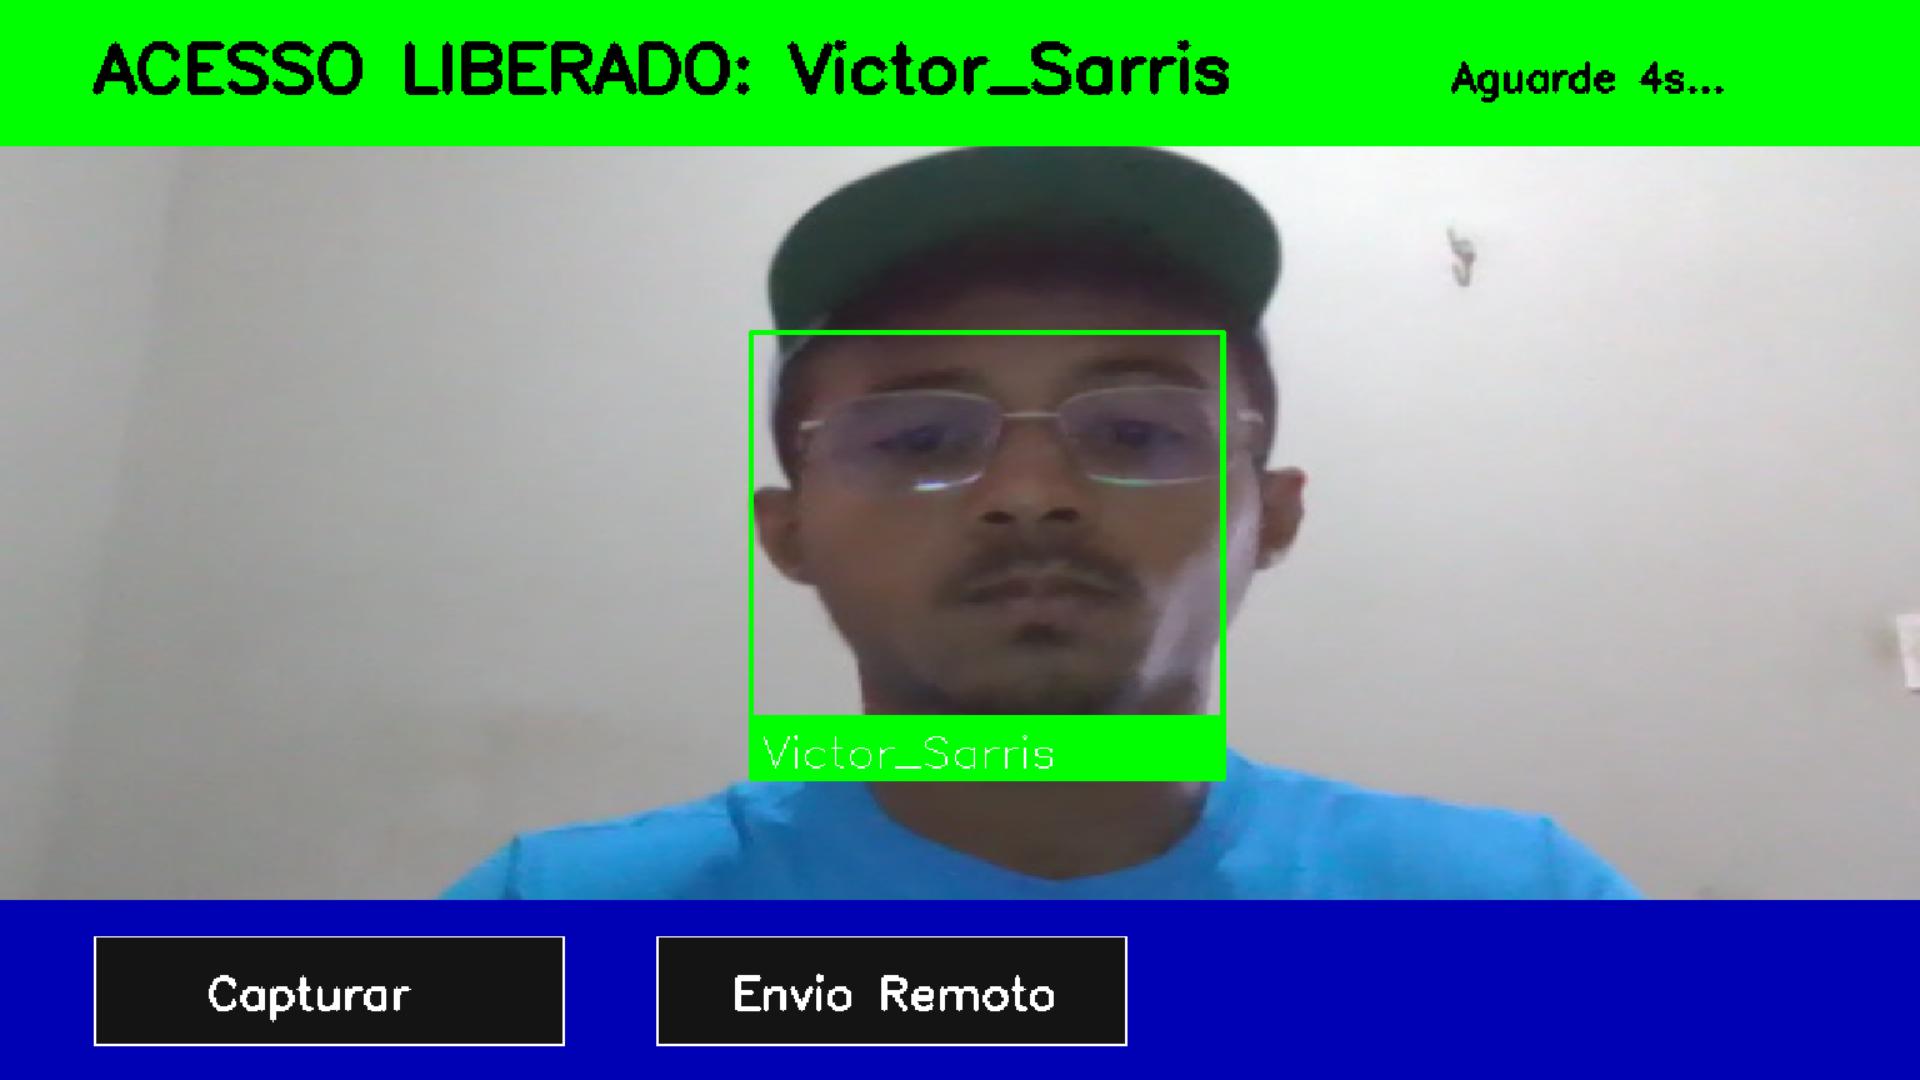
\includegraphics[width=\textwidth]{img/metodologia/reconhecimento2.png}
        \\ (b) Com boné
    \end{minipage}
    \vspace{0.3em}
    \footnotesize
    \label{fig:reconhecimento-tempo-real}
    \fonte{Elaborado pelo autor (2026).}
\end{figure}

\subsubsection{Avaliação}
\label{subsubsec:avaliacao}

A penúltima etapa afere objetivamente a eficácia do artefato através de métricas pré-estabelecidas \citeonline{peffers2007design}. A avaliação do sistema foi conduzida por meio de uma abordagem quantitativa comparativa. Primeiramente, estabeleceu-se a \textit{baseline} de desempenho a partir da coleta de dados nas três clínicas reais amostradas, documentando a latência do processo manual. Em contraste, a métrica de desempenho computacional (Performance) do totem foi registrada. O \textit{SBC} Labrador demonstrou capacidade de concluir o ciclo de inferência e validação da identidade em aproximadamente 1,3 segundos. A justaposição desses dois cenários comprova o impacto drástico do artefato proposto na redução de filas.

\subsubsection{Comunicação}
\label{subsubsec:comunicacao}

A etapa final da \textit{DSR} prevê a difusão do problema resolvido e do conhecimento gerado para pesquisadores e profissionais da área \citeonline{peffers2007design}. O esforço de comunicação científica deste projeto materializa-se por meio da redação do presente Artigo Científico e sua respectiva defesa acadêmica perante a banca examinadora do curso de Tecnologia em Análise e Desenvolvimento de Sistemas do Instituto Federal do Piauí (IFPI) - Campus Floriano. Adicionalmente, o detalhamento da arquitetura fornece um escopo documentado para futuras aplicações de Sistemas Embarcados na região.

\subsection{ANÁLISE DOS DADOS}
\label{subsec:analise-dados}

Para os dados quantitativos — compostos pelas amostras de tempo cronometrado nas três clínicas de saúde (oftalmológica, odontológica e multidisciplinar) e pelos \textit{logs} de tempo de inferência do \textit{hardware} local —, foi empregada a estatística descritiva. As cronometragens do processo manual, registradas originalmente em atas de minutos e segundos, foram tabuladas e convertidas para uma unidade de medida padronizada (segundos). Isso permitiu o cálculo das médias aritméticas de tempo de espera de cada instituição, viabilizando o contraste matemático direto contra a variável de Performance do sistema automatizado. A organização dos dados e a geração dos gráficos comparativos foram realizadas com o auxílio do \textit{software} Microsoft Excel.  

Os dados qualitativos, extraídos dos formulários de mapeamento de processos aplicados à gestão e aos atendentes, foram analisados através da técnica de análise de conteúdo. Esse método permitiu categorizar as respostas discursivas e identificar os padrões que causam os gargalos na recepção — agrupados nas categorias demora no credenciamento, tempo de cadastro e esquecimento de documentos, construídas a partir dos relatos dos atendentes da recepção nas clínicas. O cruzamento dessas informações qualitativas com os tempos elevados da estatística descritiva embasou a justificativa operacional para a implementação de um artefato tecnológico. 

\subsection{ASPECTOS ÉTICOS}
\label{subsec:aspectos-eticos}

Esta pesquisa foi conduzida em estrita observância aos princípios éticos estabelecidos pela Resolução nº 466/2012 e pela Resolução nº 510/2016 do Conselho Nacional de Saúde (CNS). É imperativo destacar que o escopo da coleta de dados em campo caracterizou-se unicamente pela observação de fluxos operacionais e pelo registro de tempos médios de atendimento, não envolvendo qualquer intervenção clínica, manipulação biológica ou coleta de dados pessoais e sensíveis dos indivíduos presentes nos estabelecimentos de saúde.  

Para o levantamento da base de dados empírica do processo de credenciamento manual, garantiu-se o anonimato absoluto. Não foram registrados nomes, diagnósticos, documentos pessoais (CPF, RG) ou imagens biométricas dos pacientes durante as cronometragens e a aplicação dos formulários de mapeamento. Adicionalmente, as próprias instituições de saúde colaboradoras foram categorizadas de forma genérica neste trabalho (por exemplo, ``Clínica Oftalmológica'' e ``Clínica Odontológica'') para salvaguardar o sigilo e a integridade institucional.  

Dada a natureza estritamente administrativa do mapeamento de processos e a total anonimização das variáveis amostrais, a etapa de campo desta pesquisa não foi submetida à avaliação do Comitê de Ética em Pesquisa (sistema CEP/Plataforma Brasil). Essa autoavaliação apoia-se nos critérios de não obrigatoriedade de registro previstos na Resolução nº 510/2016 do CNS para investigações que não envolvem identificação individual dos participantes nem coleta de dados sensíveis, reforçados pelo caráter anonimizado das variáveis coletadas (art. 12 da Lei Geral de Proteção de Dados Pessoais -- LGPD, Lei nº 13.709/2018). Ressalta-se que a dispensa formal de submissão é prerrogativa exclusiva do próprio comitê de ética; o que se apresenta aqui é a justificativa e a autoavaliação adotadas pelo pesquisador, não uma dispensa institucional automática.

Por fim, no que concerne à fase de Demonstração e Avaliação tecnológica do artefato biométrico, os testes de inferência do \textit{SBC} Labrador e a captura facial através do módulo OV2640 foram realizados em ambiente de laboratório controlado. Esta etapa contou exclusivamente com a participação voluntária da equipe de investigação e de parceiros de projeto previamente informados, assegurando que o processamento do \textit{pipeline} de Visão Computacional operasse de forma local e isolada, respeitando os preceitos globais de privacidade e a Lei Geral de Proteção de Dados Pessoais (LGPD).



\section{RESULTADOS E DISCUSSÃO}
\label{sec:resultados}

\subsection{RESULTADOS DO MAPEAMENTO OPERACIONAL}
\label{resultados-mapeamento}

A etapa de coleta empírica de dados nas três instituições de saúde do município de Floriano-PI teve como objetivo documentar o esforço operacional e humano exigido pelo método tradicional de credenciamento. Através da observação direta e da cronometragem dos atendimentos, foi possível estabelecer uma linha de base quantitativa (\textit{baseline}) sobre a eficiência do fluxo de recepção. Cabe ressaltar que o tamanho reduzido da amostra justifica-se tanto pelo curto tempo hábil para o desenvolvimento integral do projeto — delimitado a seis meses —, quanto pela recusa de outras instituições de saúde da região em autorizar a observação e a cronometragem de seus processos internos, o que restringiu a expansão do levantamento empírico.

Os dados coletados evidenciaram uma alta variância e um tempo de espera significativamente elevado para um ambiente clínico. Na Clínica Oftalmológica amostrada (que atende em média 30 pacientes por dia), foram cronometrados 4 atendimentos, cujos tempos individuais variaram de 5 minutos e 15 segundos até o pico de 7 minutos e 51 segundos. Na Clínica Odontológica, com 5 atendimentos cronometrados, a variação situou-se entre 3 minutos e 45 segundos e 6 minutos e 11 segundos. Por fim, na Clínica Multidisciplinar, também com 5 atendimentos cronometrados, os tempos flutuaram entre 3 minutos e 29 segundos e 5 minutos e 28 segundos por atendimento. No total, foram cronometrados 14 credenciamentos manuais nas três instituições. A Tabela \ref{tab:tempos_credenciamento} resume a consolidação quantitativa destas observações empíricas.

\begin{table}[H]
    \centering
    \caption{Síntese dos tempos operacionais de credenciamento manual}
    \label{tab:tempos_credenciamento}
    \small
    \begin{tabularx}{\textwidth}{>{\raggedright\arraybackslash}p{4.2cm} >{\centering\arraybackslash}p{0.8cm} >{\centering\arraybackslash}p{2.4cm} >{\centering\arraybackslash}p{2.4cm} >{\centering\arraybackslash}X}
        \toprule
        \textbf{Instituição de Saúde} & \textbf{N} & \textbf{Tempo Mínimo} & \textbf{Tempo Máximo} & \textbf{Tempo Médio Estimado} \\ 
        \midrule
        Clínica Oftalmológica & 4 & 05m 15s & 07m 51s & $\sim$ 06m 15s \\
        Clínica Odontológica & 5 & 03m 45s & 06m 11s & $\sim$ 04m 57s \\
        Clínica Multidisciplinar & 5 & 03m 29s & 05m 28s & $\sim$ 04m 40s \\
        \bottomrule
    \end{tabularx}
    \fonte{Elaborado pelo autor (2026). N = número de atendimentos cronometrados por instituição (total de 14 credenciamentos observados).}
\end{table}

Para compreender as causas fundamentais desta demora, os dados quantitativos foram cruzados com os resultados qualitativos obtidos através dos formulários aplicados aos atendentes. A análise de conteúdo das respostas revelou que a ineficiência não decorre da infraestrutura das clínicas, mas sim da natureza analógica do processo de verificação de identidade e registro.  

Questionados sobre qual etapa demanda mais tempo, os colaboradores apontaram, em todas as respostas, algum processo de natureza burocrática ou administrativa. Na Clínica Oftalmológica, o principal estrangulamento relatado foi a passagem de documentos do paciente, agravado pelo fato de que ``o paciente às vezes demora ou não entrega'' os documentos exigidos. Na Clínica Odontológica, a etapa mais lenta apontada foi a ``anamnese''. Já na Clínica Multidisciplinar, cujo formulário foi respondido por dois atendentes distintos, houve convergência quanto à natureza administrativa do gargalo, ainda que com ênfases diferentes: um dos respondentes apontou o ``cadastro'' como a etapa mais lenta, relatando que ``o cadastro é a parte que mais demora, pois os horários das profissionais são pontuais''; o outro destacou a dificuldade de ``encaixar o paciente na disponibilidade do profissional'' em razão da procura por horário disponível. Adicionalmente, os formulários demonstraram que a maioria dos atendentes (3 dos 4 respondentes) considera positiva a implementação de um sistema automatizado para mitigar a demora no credenciamento.  

Estes resultados consolidam o diagnóstico de que o modelo manual de controle de acesso não apenas consome tempo excessivo da equipe de recepção, como também é intrinsecamente dependente de variáveis não controláveis (o paciente lembrar-se de trazer o documento físico e a velocidade de digitação do atendente). É exatamente sobre este gargalo operacional — a dependência de credenciais físicas e a digitação manual de cadastros — que o artefato tecnológico desenvolvido neste trabalho atua, conforme será discutido a seguir.

\subsection{DESEMPENHO COMPUTACIONAL DO ARTEFATO (A SOLUÇÃO)}
\label{desempenho-computacional}

Em contrapartida ao cenário analógico diagnosticado, a fase de Demonstração da metodologia \textit{Design Science Research} submeteu o artefato tecnológico a testes rigorosos em ambiente de laboratório controlado. O objetivo desta etapa foi validar a responsividade do código, a estabilidade da arquitetura de hardware e, sobretudo, a relação de compromisso (\textit{trade-off}) entre o tempo de inferência da rede neural e a sua taxa de acurácia operando de forma nativa no dispositivo.  

O sistema foi concebido sob o paradigma da Computação de Borda, garantindo que todo o \textit{pipeline} de Visão Computacional operasse de forma estritamente local e \textit{offline}. Durante as simulações práticas, o fluxo de reconhecimento iniciou-se com a detecção de proximidade do usuário, validada pelo módulo de distância a laser, que por sua vez acionou o módulo de câmera OV2640 para a coleta da biometria facial.  

A carga de processamento intensivo foi direcionada ao \textit{SBC} Labrador, atuando como o núcleo computacional do totem. A análise dos registros contínuos (\textit{logs}) extraídos da \textit{API} do sistema revelou um dado crucial para a viabilidade do projeto: a capacidade do tempo de inferência compensar as margens de confiança do modelo preditivo. Os relatórios atestaram que a rede neural registrou percentuais de confiança geométrica (confianca\_pct) que variaram predominantemente de 56,42\% a 75,16\% em autenticações bem-sucedidas com acesso liberado (``LIBERADO''). Como exemplificado na imagem \ref{fig:relatorio-log}.

Cabe ressaltar que os nomes originais registrados durante a fase de testes e validação do sistema foram substituídos por identificadores genéricos (como ``Usuario1'' e ``Usuario2'') nos extratos apresentados na Figura 9. Essa etapa de anonimização foi aplicada para garantir a desvinculação absoluta das métricas de inferência à identidade dos voluntários. Ao inviabilizar a identificação dos indivíduos, assegura-se que as informações aqui publicadas não se classifiquem como dados pessoais, em estrita conformidade com a Lei Geral de Proteção de Dados Pessoais (LGPD - Lei nº 13.709/2018), cujo Artigo 12 estabelece que dados anonimizados não estão sujeitos ao seu escopo de aplicação.

\begin{figure}[H]
    \centering
    \caption{Extrato de resposta \textit{JSON} da \textit{API} detalhando as métricas de tempo, confiança e temperatura}
    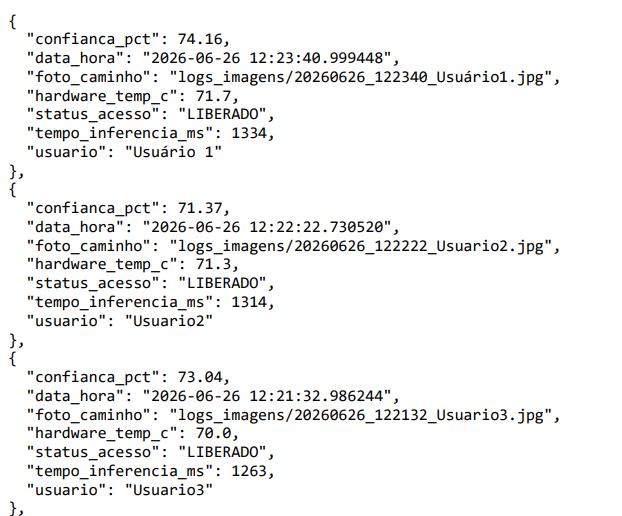
\includegraphics[width=0.7\textwidth]{img/considerações finais/relatorio-log.png}
    \fonte{Elaborado pelo Autor (2026).}
    \label{fig:relatorio-log}
\end{figure} 

Embora arquiteturas processadas em nuvem de alto custo possam apresentar limiares de confiança superiores, o modelo embarcado localmente destaca-se pela sua extrema velocidade. O tempo de inferência (\textit{tempo\_inferencia\_ms)} para extrair as assinaturas matemáticas e validar a identidade manteve-se consistente na faixa de 1253 ms a 1352 ms na grande maioria das requisições. Consolida-se, assim, a marca operacional de aproximadamente 1,3 segundos para a resolução biométrica. Cabe ressaltar que esta métrica isola estritamente o esforço computacional do \textit{hardware} — intervalo compreendido entre a captura do quadro pela câmera após o gatilho a laser e a emissão do sinal de liberação na tela —, não contabilizando o tempo prévio de deslocamento e posicionamento físico do paciente diante do sensor. Ainda assim, esta velocidade de resposta atua como um fator de compensação direta: mesmo na eventualidade de uma validação com confiança inferior que exija uma segunda aproximação do rosto, a penalidade temporal para o paciente resume-se a mais 1,3 segundos.

Outro indicador técnico de extrema relevância extraído da demonstração foi o comportamento térmico do \textit{hardware} local. O \textit{SBC} Labrador registrou temperaturas (\textit{hardware\_temp\_c)} oscilando entre 50,6 °C e picos de 75,9 °C durante as sequências de requisições intensivas da inteligência artificial. O processador suportou a carga contínua sem atingir falhas de sobreaquecimento ou \textit{throttling} severo, assegurando a confiabilidade para a operação em horário comercial. A integridade de todos estes resultados métricos (tempo, temperatura e confiança), extraídos diretamente das respostas \textit{JSON} da \textit{API} do sistema em tempo real, pode ser auditada nos extratos de \textit{logs} brutos disponibilizados no Apêndice.  

Por fim, o protótipo confirmou a viabilidade da comunicação entre os sistemas embarcados. Após a identificação validada, o \textit{software} emitiu um sinal de confirmação visual na tela \textit{IPS}, sem falhas de sincronia, acionando de imediato a liberação do acesso.  

\subsection{AVALIAÇÃO COMPARATIVA DAS HIPÓTESES}
\label{avalicao-teste}

A etapa final da avaliação no ciclo da \textit{Design Science Research} consiste em cruzar os resultados da operação manual (\textit{baseline}) com o desempenho do artefato tecnológico construído, permitindo a validação direta das hipóteses estipuladas no início deste estudo.

A Hipótese Principal (H1) propõe que o uso do sistema de controle de acesso automatizado reduziria significativamente o tempo médio de credenciamento dos pacientes, otimizando o fluxo operacional e aumentando a eficiência da recepção em comparação com o método manual. Os dados coletados apontam favoravelmente para essa premissa: enquanto o método tradicional (em ambiente clínico real, sujeito a filas, variabilidade de pacientes e imprevistos operacionais) registrou tempos de espera que atingiram até 7 minutos e 51 segundos, o totem biométrico (avaliado em ambiente de laboratório controlado, com voluntários cooperativos) demonstrou capacidade de concluir a inferência e validação da identidade em aproximadamente 1,3 segundos. É importante ressaltar, contudo, que essa comparação não decorre de um teste controlado sob as mesmas condições: os dois cenários foram mensurados em contextos distintos -- um em campo, sujeito às adversidades reais da recepção, e outro em laboratório, sob condições favoráveis — de modo que o resultado deve ser interpretado como evidência da viabilidade técnica e do potencial de ganho de desempenho do artefato, e não como uma comprovação estatística direta da redução do tempo médio de credenciamento no ambiente real. Adicionalmente, a métrica do artefato reflete o tempo de resposta do núcleo biométrico, e não o fluxo operacional ponta a ponta na clínica (que envolveria o deslocamento e posicionamento do paciente). Ainda assim, a diferença nas ordens de grandeza (minutos versus segundos) sugere fortemente a capacidade estrutural da solução em mitigar a formação de filas no balcão, hipótese que deverá ser confirmada de forma conclusiva em trabalhos futuros por meio de testes de campo controlados no próprio ambiente clínico.

A Hipótese Secundária (H2) sugeria que as redes neurais profundas (\textit{embeddings}) garantiriam uma elevada taxa de precisão, mitigando vulnerabilidades como a perda ou compartilhamento de forma indevida de credenciais físicas. O cruzamento qualitativo revelou que o maior estrangulamento operacional, segundo os próprios atendentes, era justamente o fato de que ``o paciente às vezes demora ou não entrega'' os documentos físicos. A adoção da assinatura matemática facial contorna definitivamente este problema: a credencial passa a ser o próprio rosto do indivíduo, intransferível e imune a esquecimentos. Aliada às consistentes margens de confiança preditiva registradas de forma autônoma pelo \textit{SBC} Labrador (entre 56,42\% e 75,16\% para acessos liberados), a H2 é confirmada. 

Por fim, a Hipótese Secundária (H3) propõe que a adoção biométrica eliminaria a necessidade de interação física com superfícies ou funcionários, promovendo um ambiente clínico biologicamente mais seguro. A arquitetura de \textit{hardware} validou diretamente este ponto: a integração do sensor de distância a laser VL53L0X atua como um gatilho automático. Perante a simples aproximação do usuário, a câmera OV2640 é ativada para realizar a leitura facial, dispensando de forma absoluta o toque em telas (\textit{touchscreens}) ou o manuseio de papéis e cartões na recepção. A premissa de um credenciamento totalmente \textit{contactless} comprova, portanto, a H3.  

Em suma, os dados quantitativos e qualitativos atestam que o totem biométrico gerido soluciona com eficácia a lentidão e a insegurança inerentes ao controle de acesso manual, cumprindo integralmente os objetivos traçados para esta investigação tecnológica.

\section{CONSIDERAÇÕES FINAIS}
\label{sec:consideracoes-finais}

O presente artigo teve como objetivo central desenvolver e avaliar um artefato tecnológico de reconhecimento facial baseado em arquitetura de Computação de Borda para automatizar o processo de credenciamento de pacientes em ambientes de saúde, visando reduzir o tempo de espera e mitigar falhas operacionais.  

Através da aplicação da metodologia \textit{Design Science Research} (DSR), conclui-se que a adoção da tecnologia biométrica no fluxo de recepção atinge plenamente os propósitos estabelecidos. Os resultados empíricos da fase de demonstração revelaram que o modelo tradicional analógico consome um tempo excessivo da equipe de recepção — atingindo picos de quase 8 minutos por atendimento —, além de fragilizar a experiência do paciente devido a esquecimentos de documentos e procedimentos burocráticos repetitivos.  

Em resposta a esse cenário, o totem biométrico desenvolvido provou que a automação mitiga diretamente essas falhas operacionais. A arquitetura de hardware concebida, fundamentada em um \textit{SBC} Labrador operando em conjunto com sensores de proximidade (VL53L0X) e um módulo ESP32-CAM, validou a aplicabilidade do paradigma da Computação de Borda no setor da saúde. O sistema demonstrou capacidade para executar rotinas complexas de redes neurais profundas de forma local, \textit{offline} e autônoma, garantindo a extração de \textit{embeddings} e a liberação de acesso na marca de 1,3 segundos, sem comprometer a estabilidade térmica do equipamento ou a privacidade dos dados do paciente. 

Portanto, a implementação do sistema atende com êxito ao objetivo traçado ao converter um procedimento presencial demorado em uma validação sem contato de pouco mais de um segundo, eliminando estruturalmente as filas de espera e reduzindo o erro humano associado à verificação de identificações físicas.  

Embora o protótipo tenha alcançado pleno êxito laboratorial e demonstrado a viabilidade das hipóteses levantadas, este estudo apresenta delimitações inerentes à janela de desenvolvimento de seis meses e às restrições de autorização institucional. A amostra da \textit{baseline} restringiu-se a três clínicas devido à recusa e indisponibilidade de outras instituições. Além disso, por restrições de prazo e de trâmites de aprovação ética para testes com pacientes reais, o artefato tecnológico foi validado em um ambiente de laboratório controlado, contrastando com a \textit{baseline} medida no cenário clínico não controlado. A operação do sistema também focou-se estritamente no fluxo de Identificação (1:N) sobre a base de dados de pacientes previamente cadastrados no dispositivo. Por fim, reconhece-se como limitação adicional o fato de o artefato não ter sido submetido a testes de desempenho segmentados por condições de iluminação, tons de pele, gênero ou faixa etária dos usuários -- fatores de variação de acurácia amplamente documentados na literatura de reconhecimento facial --, de modo que a generalização da precisão observada para diferentes condições de captura e subgrupos populacionais não pôde ser verificada neste estudo, permanecendo como recomendação prioritária para trabalhos futuros antes de qualquer implantação em produção.  

Como sugestão para trabalhos futuros, recomenda-se a implementação de algoritmos de prova de vida no processamento visual para mitigar tentativas de fraude com apresentação de fotografias impressas ou em telas. Adicionalmente, o desenvolvimento de uma interface de sincronização em nuvem robusta (\textit{API RESTful} bidirecional) para integrar o totem de forma nativa com Sistemas de Informação Hospitalar comerciais expandiria o alcance prático da solução. Em suma, o artefato gerado consolida a premissa de que a engenharia de sistemas embarcados e a inteligência artificial possuem um potencial técnico maduro para revolucionar a gestão de processos operacionais na área da saúde.  


% Os itens de Cronograma e Recursos (geralmente presentes em Projetos de Pesquisa) 
% foram comentados ou embutidos como subseções/comentários para preservar a estrutura de Artigo Científico.
% Em Artigos (resultados finais), o foco recai sobre Discussão dos Resultados.



% ========================================================================
% ELEMENTOS PÓS-TEXTUAIS
% ========================================================================
% ========================================================================
% ELEMENTOS PÓS-TEXTUAIS
% Referências, apêndices e anexos conforme ABNT NBR 14724:2011
% ========================================================================

% ========================================================================
% REFERÊNCIAS BIBLIOGRÁFICAS
% ========================================================================
\postextual

% Configura o título das referências
\bibliography{referencias}

% ========================================================================
% GLOSSÁRIO (OPCIONAL)
% ========================================================================
% Descomente se necessário incluir glossário
% \glossary

% ========================================================================
% APÊNDICES (OPCIONAL)
% ========================================================================
% Descomente e personalize se houver apêndices
% Os apêndices são textos elaborados pelo próprio autor

\begin{apendicesenv}
    % Imprime uma página indicando o início dos apêndices
    % \partapendices
    
    % ========================================================================
    % APÊNDICE A - EXEMPLO DE APÊNDICE
    % ========================================================================

    \begin{figure}[H]
        \textbf{APÊNDICE A – EXTRATOS DOS LOGS DE AUDITORIA DA API}
        \centering
        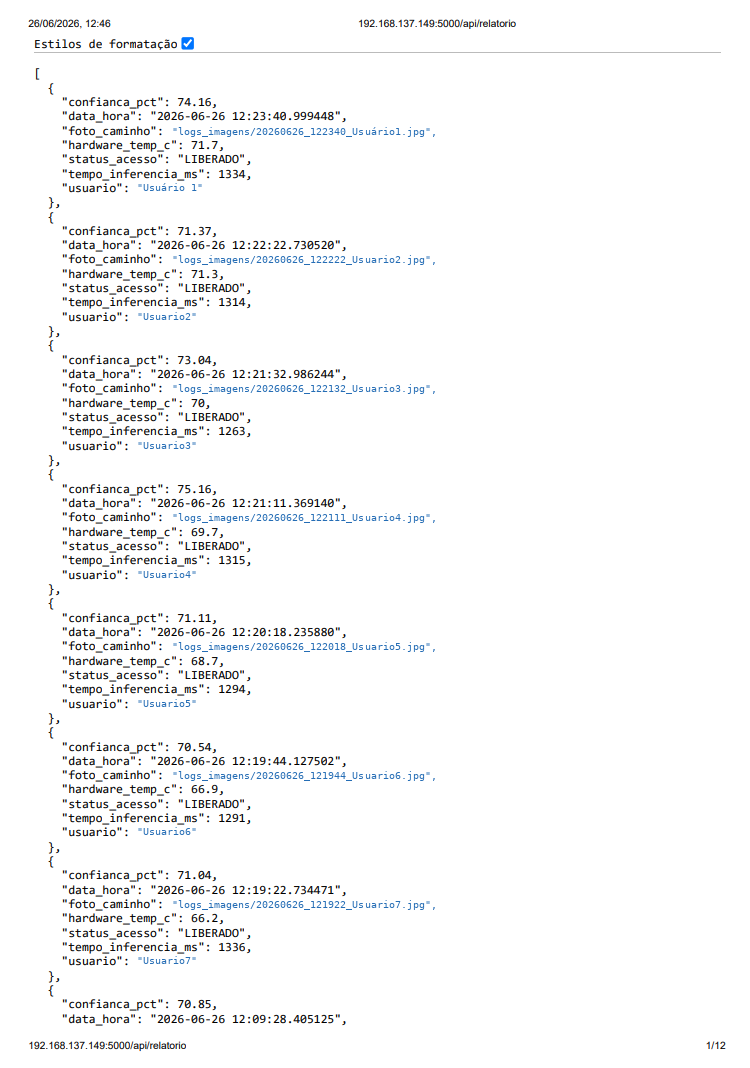
\includegraphics[width=1\textwidth]{img/apendice/folha de relatorio 1 (anonimizada).png} 
        \vspace{0.3em}
        \footnotesize 
        \label{fig:folha-relatorio1}
    \end{figure}
    \begin{figure}[H]
        \textbf{APÊNDICE B - REGISTRO BRUTO DE CRONOMETRAGEM DOS ATENDIMENTOS NAS CLÍNICAS AMOSTRADAS}
        \centering
        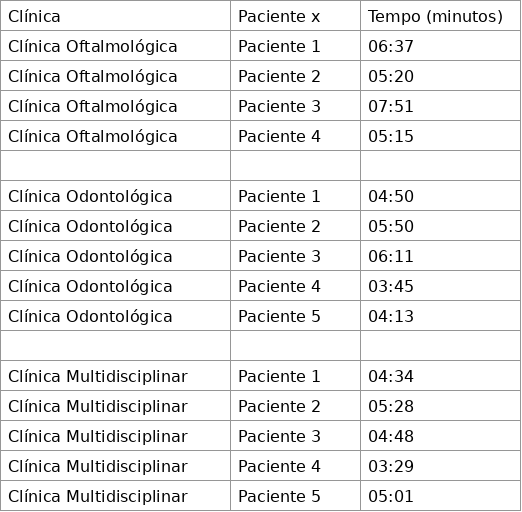
\includegraphics[width=1\textwidth]{img/apendice/tempo-conometrado.png} 
        \vspace{0.3em}
        \footnotesize 
        \label{fig:folha-relatorio1}
    \end{figure}
    \begin{figure}[H]
        \textbf{APÊNDICE C - EXTRATO DAS RESPOSTAS AO FORMULÁRIO DE MAPEAMENTO DE PROCESSOS}
        \centering
        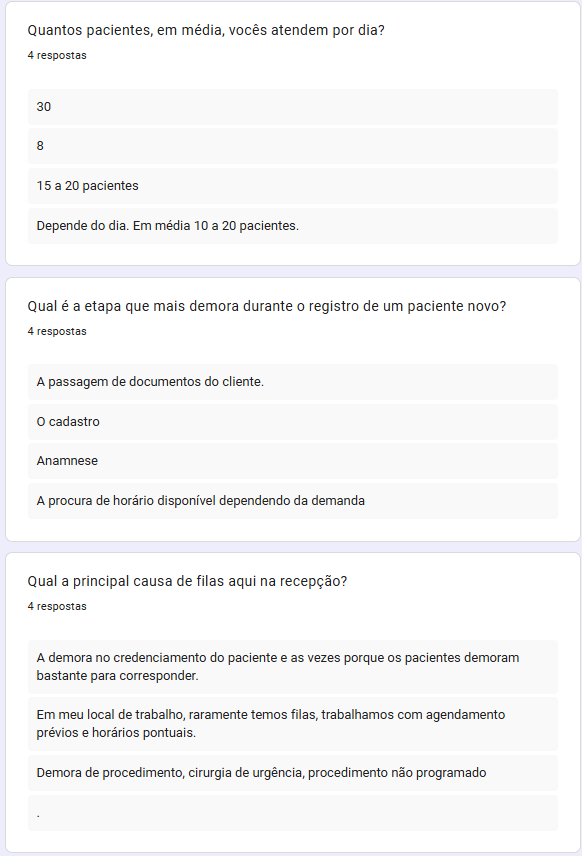
\includegraphics[width=1\textwidth]{img/apendice/mapeamento-processos1.png} 
        \vspace{0.3em}
        \footnotesize 
        \label{fig:folha-relatorio1}
    \end{figure}
    \begin{figure}[H]
        \centering
        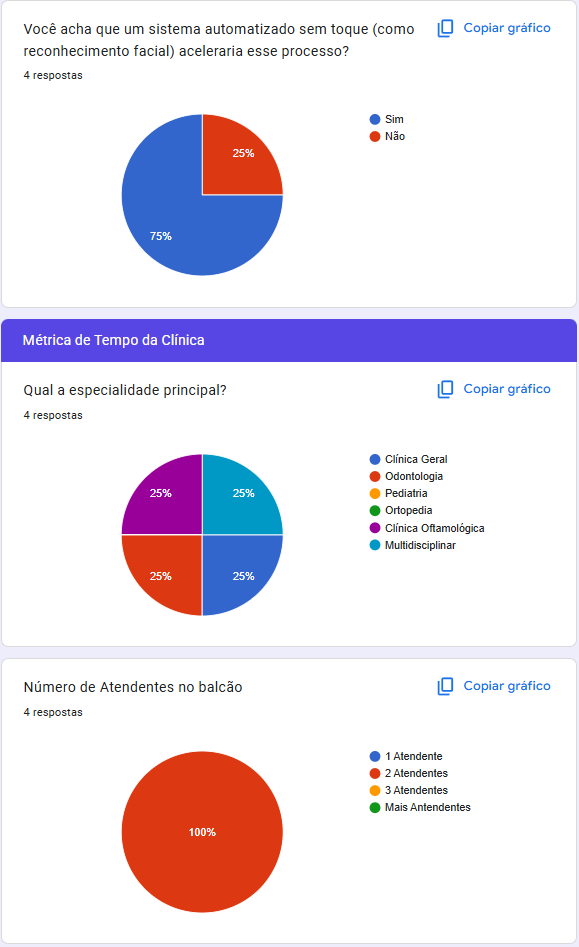
\includegraphics[width=1\textwidth]{img/apendice/mapeamento-processos2.png} 
        \vspace{0.3em}
        \footnotesize 
        \label{fig:folha-relatorio1}
    \end{figure}
    \begin{figure}[H]
        \centering
        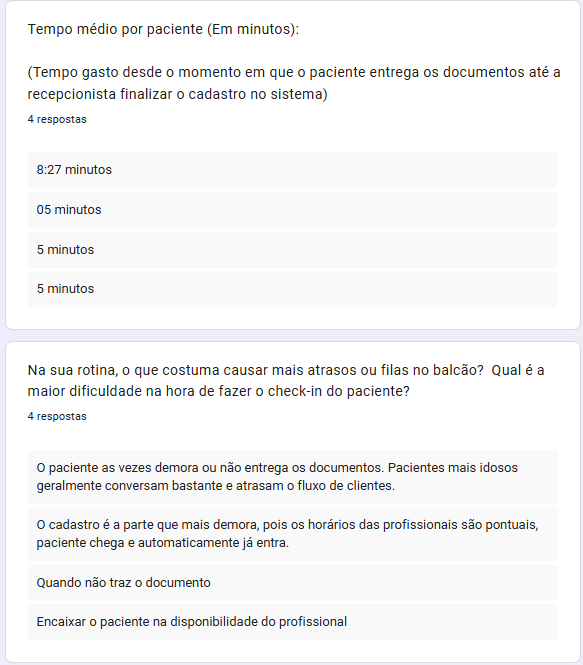
\includegraphics[width=1\textwidth]{img/apendice/mapeamento-processos3.png} 
        \vspace{0.3em}
        \footnotesize 
        \label{fig:folha-relatorio1}
    \end{figure}
    \textbf{APÊNDICE D - DOCUMENTAÇÃO DO PROJETO} \\
    \url{https://face-recognition-totem.netlify.app/#} \\
    \url{https://github.com/Victor-Sarris/Totem-Reconhecimento-Facial}
\end{apendicesenv}


% ========================================================================
% FIM DO DOCUMENTO
% ========================================================================
\end{document}
